\documentclass[11pt]{article}

\usepackage[review]{acl}
\usepackage{times}
\usepackage{latexsym}
\usepackage[T1]{fontenc}
\usepackage[utf8]{inputenc}
\usepackage{microtype}
\usepackage{inconsolata}
\usepackage{booktabs}
\usepackage{graphicx}
\usepackage{array}
\usepackage{tabularx}
\usepackage{enumitem}
\usepackage{placeins}
\usepackage{amsmath}
\usepackage{amsfonts}
\usepackage{amssymb}
\usepackage{forest}
\usepackage{tikz}
\usetikzlibrary{arrows.meta,calc,positioning}
\setlength{\emergencystretch}{3em}
\setlength{\linenumbersep}{6pt}

\title{When Are Robust-RAG Results Comparable?\\
A Two-Layer Estimand Audit}
\author{Anonymous Authors}
\date{}

\begin{document}
\maketitle

\begin{abstract}
Robust retrieval-augmented generation (RAG) papers often share labels such as
noise robustness, faithfulness, security, or calibration while answering
different decision questions. We introduce a two-layer estimand audit. The
substantive layer aligns evidence state, origin/capability, intervention,
outcome, and policy/utility; the measurement layer aligns items, reviewers,
treatment assignment, references, and downstream loss. In a fixed audit of 39
venue-linked robust-RAG papers with local full text, nine collect original
human judgments. Only two report the number of distinct annotators, and none
reports item--annotator assignment; because none randomizes reviewer prompts,
we identify reporting gaps rather than a confirmed unit error. A
consequence-defined 480-item test also finds no uniform advantage from adding
explicit capability and utility prompts across three open models. Finally, in
5,000 sharp-null simulations with moderate reviewer heterogeneity, a
source-only test of panel-majority correctness rejects 17.0\% of the time. An
oracle randomization test using the identical statistic rejects 5.3\%;
doubling sources raises the former to 25.9\% while the latter remains 4.9\%.
An unreliable development diagnostic and an unverifiable human collection are
not used as validation. We release source-linked audits, model outputs, and
the same-statistic simulation. More judged items cannot replace independently
assigned reviewers.
\end{abstract}

\section{Introduction}

Robust RAG studies operate under irrelevant, insufficient, conflicting, stale,
weakly sourced, or malicious evidence. Two reported ``robustness'' gains may
nevertheless concern different retrieval snapshots, attacker capabilities,
interventions, outcome units, or deployment actions. Source verification is
therefore necessary but insufficient: a cross-paper claim must also establish
that both results answer a compatible decision question.

Evaluating that compatibility creates a second estimand problem. If an audit
prompt is assigned to six people but hundreds of their labels are analyzed
only by item or source, the apparent sample size concerns repeated judgments,
not treatment assignments. If a reference rubric repeats the concepts
foregrounded by one prompt, agreement measures similarity to that
construction rather than independent criterion validity. These consequences
follow from crossed participant--item designs, clustering, and reference
construction \citep{baayen2008crossed,barr2013maximal,abadie2023clustering}.
We make them operational for robust-RAG claim review.

This paper makes three contributions. First, it defines a two-layer audit:
five substantive coordinates determine what system comparison is proposed,
and five measurement objects determine what a claim-review experiment
estimates. Representative robust-RAG boundary cases motivate the coordinates;
the literature map is documentary context rather than a census. Second, a
source-linked audit applies the measurement layer to nine published
human-judgment studies, while a controlled 480-item experiment tests the two
decision coordinates on three open models. Both are deliberately diagnostic:
they expose reporting gaps and model dependence rather than validate the
framework. Third, a parameterized null simulation compares source-only and
assignment-aware references using the \emph{same} panel-majority statistic,
isolating uncertainty from reviewer assignment.

Our hard conclusion is narrow. When treatment is assigned to reviewers,
adding items cannot justify item-only uncertainty for a reviewer-population
effect. The substantive coordinates remain candidate disclosures, not a
validated human instrument. We also distinguish public de-identification from
private auditability: identity-bearing recruitment and consent records may
remain access-controlled, but an empirical claim still needs an inspectable
internal provenance path.

\section{Positioning}
\label{sec:related}

\paragraph{RAG surveys and shared evaluation.}
General surveys organize RAG architectures and applications, while evaluation,
trustworthiness, security, conflict, and abstention surveys expose different
failure surfaces \citep{ragSurvey2024,ragEvaluationSurvey2024,
trustRAGCompass2024,securityRAGSurvey2026,xuKnowledgeConflicts2024,
wenAbstentionSurvey2025}. Common-harness comparisons improve empirical
control \citep{ragBestPractices2024,alushiRAGComparison2026}, but they do not
resolve whether a quoted cross-paper result concerns the same evidence state,
capability envelope, outcome, or action. Table~\ref{tab:main-prior-work-comparison}
positions our claim-level comparison lens alongside these lines.

\begin{table*}[t]
\centering
\footnotesize
\renewcommand{\arraystretch}{0.92}
\begin{tabularx}{\linewidth}{>{\raggedright\arraybackslash}p{0.18\linewidth}>{\raggedright\arraybackslash}p{0.22\linewidth}>{\raggedright\arraybackslash}p{0.25\linewidth}X}
\toprule
\textbf{Adjacent line} & \textbf{Primary unit} &
\textbf{Unresolved comparison question} & \textbf{This paper's increment} \\
\midrule
General RAG surveys \citep{ragSurvey2024,ragComprehensive2025} &
Architectures, modules, applications &
Whether similarly named gains concern the same evidence state, outcome, and
experimental game &
Adds a claim-level comparison lens and an estimand audit; does not claim a
venue-complete census. \\
Evaluation surveys and unified comparisons
\citep{ragEvaluationSurvey2024,ragBestPractices2024,
alushiRAGComparison2026} &
Metrics, benchmarks, and common-harness reruns &
Which controls are required by a specific cross-study or mechanistic
inference when rerunning is impossible &
Separates scientific coordinates from assignment, participant, item, and
reference units; the simulation quantifies one resulting failure mode. \\
Trustworthy and security RAG surveys
\citep{trustRAGCompass2024,trustworthyRAGSurvey2025,securityRAGSurvey2026} &
Trust dimensions, attack surfaces, and defenses &
Whether benign conflict and attacker-created corruption share a transferable
capability envelope &
Makes origin/access/budget explicit and shows why a prompt-overlapping
reference cannot establish independent criterion validity. \\
Conflict and abstention surveys
\citep{xuKnowledgeConflicts2024,wenAbstentionSurvey2025} &
Conflict types and refusal behavior &
Whether a confidence or sufficiency signal identifies the action that
maximizes utility at a matched operating point &
Separates signal, action, and utility and releases a consequence-defined
counterfactual target without claiming an evaluated policy. \\
\bottomrule
\end{tabularx}
\caption{Positioning relative to adjacent surveys and empirical comparison
work. Each adjacent line partitions the literature by mechanism, which is what a
reader needs to \emph{find} related work. None partitions the
\emph{comparison}, which is what a reader needs when two numbers appear
together, and none is accompanied by evidence that its categories can be read
off a paper. The increment is a reporting-coordinate reduction that is tested
(\S\ref{sec:tested}) and applied at scale (\S\ref{sec:applied}); it is not a
venue-complete systematic review, and it does not supersede these surveys for
discovery.}
\label{tab:main-prior-work-comparison}
\end{table*}


\paragraph{Human judgments as measurements.}
Annotation research distinguishes reproducibility from truth
\citep{artstein2008intercoder}. Majority voting can erase structured variation
\citep{plank2022labelvariation,davani2022disagreements}, while annotator models
retain rater and item effects \citep{passonneau2014annotation,
paun2018bayesian}. Crossed participant--item designs require both sources of
variation \citep{baayen2008crossed}, and clustering follows treatment
assignment rather than row count \citep{abadie2023clustering}. We apply these
established principles to claim-review experiments; the new contribution is
the robust-RAG synthesis and executable design stress test.

\section{Substantive Comparability in Robust RAG}
\label{sec:robust-rag-landscape}

We use the literature map as a source of boundary cases, not as prevalence
evidence. Five \emph{operating questions} organise discovery: how evidence is
constructed, how a model uses it, how deliberate corruption changes the game,
how signals become actions, and how those actions are evaluated. They are a
different cut of the same literature from the four failure surfaces of
\S\ref{sec:taxonomy}, and both are different again from the five
\emph{reporting coordinates} of \S\ref{sec:coordinates}, which describe not a
literature but a single proposed contrast. The boundary cases below are what
made the coordinates necessary.

\paragraph{Evidence availability is not evidence use.}
Irrelevant-context studies test whether retrieved distractors redirect a
generator \citep{irrelevantContext2023}; noise-aware training changes the
generator's training distribution \citep{raat2024}; RGB supplies diagnostic
stress conditions \citep{rgb2023}; and Chain-of-Note changes how retrieved
documents are read \citep{chainOfNote2023}. A filter, a trained reader, and a
benchmark may share a harness, but their native scores do not rank
interchangeable interventions. Insufficient evidence creates another
boundary: when no passage can support an answer, re-retrieval or abstention
can dominate better distractor resistance \citep{sufficientContext2024}.

\paragraph{Support, authority, conflict, and attack are distinct.}
RAGTruth annotates unsupported spans, while evaluators estimate claim or
response support \citep{ragTruth2024,ragas2024,ares2024}; knowledge-conflict
methods instead study competition between parametric memory and retrieved
evidence \citep{tugOfWar2024,faithfulRAG2025,astuteRAG2025}. A response can be
correct but unsupported, or faithful to a weak source. Provenance and timestamp
determine which source should govern \citep{kilt2021,freshllms2024,
realtimeQA2023}. Deliberate corruption changes the game again: corpus
poisoning, indirect prompt injection, and backdoors differ in corpus write
access, query knowledge, retriever visibility, insertion budget, persistence,
and objective \citep{poisonedRAG2024,aip2025,phantom2024}, and their defenses
prevent, detect, certify, trace, quarantine, or recover under different
assumptions \citep{certifiedRAG2024,rrag017,rrag128}. An attack-success
comparison is transportable only within a matched capability envelope.

\paragraph{A signal is not a policy.}
Calibration predicts a property of a score \citep{guo2017calibration};
selective prediction trades coverage against risk
\citep{geifman2017selective}; sufficient-context classification
asks whether available passages can support an answer; adaptive retrieval
chooses whether to search, verify, answer, or abstain
\citep{calibRAG2025,sufficientContext2024,whenToRetrieve2024}. Self-RAG, CRAG,
and CtrlA expose this policy layer explicitly
\citep{selfRAG2023,crag2024,ctrla2025}. Comparing them requires a common
action set, budget, and loss: accuracy alone cannot price extra retrieval,
coverage, or refusal.

\paragraph{Comparison ladder.}
The strongest contrast reruns alternatives with the same corpus snapshot,
retriever, generator, evidence state, capability envelope, action set, and
outcome. When that is impossible, synthesis should retain only the common
scope supported by both studies. If a decision-critical field is absent, the
comparison is under-specified rather than evidence that either method is
better. Appendix~\ref{sec:extended-survey} gives paper-level contrasts and the
documentary-map boundary; the next section turns these recurring boundaries
into a claim-level audit.


\section{A Two-Layer Estimand Audit}
\label{sec:estimands}

The substantive layer records five coordinates for each side of a comparison:
evidence state, origin/capability, intervention, outcome, and policy/utility,
followed by claim-specific controls
(Table~\ref{tab:main-framework-overview}). These coordinates specialize
existing distinctions from evidence synthesis, selective prediction, and
security evaluation \citep{richardson1995pico,chow1970reject,
papernot2018sok}; they are prompts for inspection, not validated primitives.
The measurement layer then asks how judgments about those coordinates were
produced: which people, items, assignments, references, and downstream losses
define the target. Passing one layer cannot repair failure in the other.

\begin{table*}[t]
\centering
\small
\renewcommand{\arraystretch}{0.92}
\begin{tabularx}{\linewidth}{>{\raggedright\arraybackslash}p{0.13\linewidth}>{\raggedright\arraybackslash}p{0.25\linewidth}>{\raggedright\arraybackslash}p{0.30\linewidth}X}
\toprule
\textbf{Field} & \textbf{Question} & \textbf{Representative values} & \textbf{Why it changes a comparison} \\
\midrule
Evidence state & What is observable at the decision boundary? & Supported; distracting; insufficient; conflicting; stale/weak provenance; adversarially manipulated; not evidence-conditioned. & Query ambiguity and model uncertainty are not silently mixed with properties of retrieved evidence. \\
Origin / capability & How did that state arise, and what can an attacker observe or change? & Benign retrieval; constructed stressor; natural drift/conflict; distribution shift; attacker-created evidence with access, budget, and target. & Transfer depends on the data-generating process and the attacker's capability envelope. \\
Intervention & What part of the system changes? & Corpus/index; retriever; reranker; context assembly; generator; verifier; system control; evaluation artifact. & Components may be alternatives in a shared harness or complementary stages in a pipeline. \\
Outcome & What object and unit are measured? & Answer correctness; retrieval quality; claim support; attack success; privacy leakage; calibration; selective risk; cost. & Identically named datasets do not make different target quantities interchangeable. \\
\textbf{Policy / utility} & What response is selected, under which costs and stakes? & Answer; verify; re-retrieve; expose conflict; clarify; quarantine; recover; abstain; coverage--risk utility. & A signal becomes operational only through an action set and a declared utility context. \\
\midrule
Control check & Does the experiment support the intended inference? & Dataset and corpus snapshot; retriever; top-$k$; generator; decoding; budget; baselines; uncertainty. & Tuple compatibility alone cannot remove experimental confounding. \\
\bottomrule
\end{tabularx}
\caption{The diagnostic schema. The five fields identify whether two results address a compatible question; a claim-specific control check then determines whether their reported numbers support the intended inference. The fields are not assumed orthogonal or sufficient.}
\label{tab:main-framework-overview}
\end{table*}


\paragraph{Three targets.}
A majority-label difference for two realized reviewer panels is a
\emph{panel contrast}. A prompt effect over reviewers instead averages
individual potential judgments over a defined participant and item
population. A claim of better decisions requires a third target: expected
downstream loss for accepting, narrowing, rejecting, or deferring a
comparison. These targets coincide only under assumptions that should be
stated rather than inherited from the aggregation rule. Appendix
Section~\ref{sec:estimand-formalization} gives the notation.

\paragraph{Assignment alignment.}
Source resampling with reviewers fixed measures item variation conditional on
the realized panel. If prompts are assigned to reviewers, reviewer-composition
variation remains even as the number of claims grows. The analysis must
therefore follow the assignment mechanism or explicitly model crossed
reviewer and item effects. More labels per person improve conditional
precision; they do not create new prompt assignments.

\paragraph{Reference independence.}
Blinding reference writers to arm responses prevents direct copying, but a
rubric that paraphrases the tested prompt still incorporates the intervention.
Adjudication then selects one hard target from a distribution of judgments.
We use ``reference-relative agreement,'' reserving ``accuracy'' for an
intervention-independent criterion and retaining disagreement whenever the
task admits multiple defensible labels.

\section{Published Human-Evaluation Reporting Audit}
\label{sec:published-audit}

To connect the measurement audit to published robust-RAG practice, we fixed a
source-linked reporting audit. Of 39 venue- or proceedings-linked Map B papers
with locally extracted full text, a deterministic human-judgment term screen
flagged 19. Full-text eligibility review retained nine papers that collected
original human judgments for benchmark construction, metric validation, error
analysis, or output evaluation. The released ledger records the exact text
lines supporting every coding decision.

\begin{table}[t]
\centering\footnotesize
\setlength{\tabcolsep}{4pt}
\begin{tabular}{lrrrr}
\toprule
Reporting field & R & P & NR & N/A \\
\midrule
Distinct annotator count & 2 & 0 & 7 & 0 \\
Raters per item & 2 & 2 & 5 & 0 \\
Item--annotator assignment & 0 & 0 & 9 & 0 \\
Aggregation rule & 1 & 2 & 6 & 0 \\
Rater agreement/uncertainty & 4 & 0 & 5 & 0 \\
Recruitment or qualifications & 5 & 1 & 3 & 0 \\
Compensation & 2 & 0 & 6 & 1 \\
Disagreement/reference resolution & 2 & 1 & 6 & 0 \\
\bottomrule
\end{tabular}
\caption{Reporting audit of nine published robust-RAG studies that collected original human judgments, identified from 39 venue-linked Map B papers with local full text (19 passed the term screen). R/P/NR denote reported, partly reported, and not reported. None randomised an audit prompt across annotators, so we found no verifiable assignment-unit mismatch. Missing fields are reporting gaps, not evidence of design errors.}
\label{tab:published-human-evaluation-audit}
\end{table}


Only two of nine papers report the number of distinct annotators; two fully
report raters per item, and none reports the item--annotator assignment.
Four report an agreement or rater-uncertainty quantity, and two report
compensation. None randomizes an audit prompt across annotators, so this audit
finds no verifiable assignment-unit mismatch. We classify absent fields as
reporting gaps rather than inferring that an unreported practice was absent or
incorrect. The fixed screen is narrow and single-coded; it establishes
concrete reporting cases, not field prevalence. The case ledger appears in
Appendix Table~\ref{tab:published-human-evaluation-cases}.

\paragraph{What the cases permit.}
The ledger distinguishes incomplete reporting from a demonstrated error.
FaithEval states that three Mechanical Turk workers judge each pair and that
majority agreement controls inclusion \citep{rrag040}. RAGTruth states that
two annotators label each response, a third reviews substantial differences,
and vendor annotators receive \$25 per hour \citep{ragTruth2024}. ParamMute
reports six senior researchers and a multiply annotated 100-item subset but
not how those researchers were allocated to items \citep{rrag024}.
PoisonedRAG identifies authors as the human evaluators but gives no
reviewer-level multiplicity \citep{poisonedRAG2024}. These examples support
specific transparency claims; they do not justify reconstructing hidden
assignments or declaring any analysis invalid. They also show why releasing
only a final majority label is insufficient for later assignment-aware
reanalysis.

\subsection{Development and provenance boundaries}

In a separate development diagnostic, three coders reviewed 80 comparison
claims and a fourth adjudicated them with model labels hidden. Only 39/80
verdicts were unanimous, pairwise \(\kappa\) ranged from .258 to .525, and the
full rule and its C2/C5 ablation each matched the adjudicated reference on
40/80 claims. The sample overlaps codebook development and has a recoverable
selection rule for only 16 items, so it demonstrates unreliability of this
workflow rather than prompt utility (Appendix
Table~\ref{tab:main-human-validation}).

A later 480-claim protocol is retained only as a design case. One returned
batch contained shared response payloads, and a later export could not be
linked to controlled recruitment records, one-to-one pseudonym mappings, and
separate response receipts available to the research team or an authorized
auditor. Public identity disclosure is neither required nor desirable: a
privacy-compatible package may release only de-identified ratings and
aggregate provenance while keeping consent, qualification, payment or
affiliation, and identity-linkage records access-controlled. Because the
necessary internal audit trail was absent here, we exclude every response,
contrast, reference statistic, participant attribute, and timing claim. The
retained 80-claim diagnostic has a project-owner attestation that four
distinct human contributors consented and were compensated; the release does
not independently verify contributor-level records, and development overlap
still prevents validation claims.

\section{A Controlled Consequence Test}
\label{sec:controlled-models}

We next test the two least conventional coordinates without using a human
reference. A deterministic benchmark contains 480 synthetic deployment
decisions in 240 counterfactual pairs. In half, only whether deployment
origin/access/budget falls inside the evaluated capability envelope changes
(C2); in half, only error-versus-abstention costs change (C5). The target is
the unique minimum of the displayed loss over \texttt{deploy\_A},
\texttt{deploy\_B}, and \texttt{defer}. Three fixed open models see every item
under crossed prompts: an ablation asks for evidence state, intervention,
outcome, controls, and action, while the full prompt explicitly adds
origin/capability and policy/utility checks. Decoding is greedy. Two
format-only pilot runs were used to replace an ambiguous output schema and
freeze single-token parsing; benchmark items, targets, and the substantive
prompt contrast were unchanged. A subsequent audit found that the initial C2
generator also changed defer cost. We fixed that cost within each pair and
reran every reported model; the resulting experiment is diagnostic, not
preregistered confirmatory evidence. In C5, defer is a displayed deterministic
function of deployment losses and is never optimal; the exogenous
manipulations are only error and abstention costs.

\begin{table}[t]
\centering\footnotesize
\setlength{\tabcolsep}{4pt}
\begin{tabular}{lrrr}
\toprule
Model & Abl. & Full & $\Delta$ \\
\midrule
Qwen2.5-7B & 53.3\% & 51.2\% & -2.1 pp \\
Phi-4-mini & 65.4\% & 68.8\% & +3.3 pp \\
OLMo-2-7B & 37.5\% & 37.5\% & +0.0 pp \\
\bottomrule
\end{tabular}
\vspace{3pt}
\begin{tabular}{lrrr}
\toprule
Model & Abl. pair & Full pair & $\Delta$ regret \\
\midrule
Qwen2.5-7B & 9.2\% & 3.8\% & +0.011 \\
Phi-4-mini & 31.2\% & 37.9\% & -0.015 \\
OLMo-2-7B & 0.0\% & 0.0\% & +0.000 \\
\bottomrule
\end{tabular}
\caption{Controlled crossed model-judge experiment. Targets are unique minima of displayed deployment losses, not expert labels. Pair columns require both members of a counterfactual pair to be correct; negative $\Delta$ regret favors the full prompt. Results describe these fixed models and items and do not imply generalisation to humans or a model population.}
\label{tab:controlled-model-judges}
\end{table}


The full prompt is not uniformly better. Exact agreement changes from
53.3\% to 51.2\% for Qwen2.5-7B, from 65.4\% to 68.8\% for Phi-4-mini, and
remains 37.5\% for OLMo-2-7B. Mean regret likewise improves only for Phi
(\(-.015\)) and worsens for Qwen (\(+.011\)); counterfactual-pair consistency
is low for all three fixed models. Phi's gain is concentrated in the C2
capability shift (\(+6.7\) points) and is zero on C5 exact agreement; Qwen
instead loses 3.7 points on C2, and OLMo emits the same decisions under both
prompts. Thus, explicitly naming a coordinate can change behavior without
reliably improving it. These outcomes provide executable construct evidence
that C2/C5 can alter a deployment target, but no general prompt advantage and
no validation for human auditing or natural paper prose. Appendix
Table~\ref{tab:controlled-model-judges-strata} gives the C2/C5 split.

\section{Null Simulation of the Assignment Mismatch}
\label{sec:simulation}

\subsection{Design}

We simulate the planned primary D--C contrast---12 of the 24 planned auditor
slots---without using any excluded outcome. Reviewers are randomly divided six
per prompt. Each source contributes six claims; each claim is rated by a
balanced three-of-six panel in both arms.
Baseline agreement is 75\%. Source and claim logit standard deviations are
.15 and .35. Reviewer abilities are 12 fixed normal quantiles with
\(\sigma_r\in\{0,.10,.20,.30\}\) on the logit scale. The true prompt effect is
zero.

For each scenario, 5,000 replicates compare three analyses. The first is a
paired source \(t\) test on panel-majority correctness. The second refers that
\emph{same studentized panel-majority statistic} to all
\(\binom{12}{6}=924\) reviewer assignments. It is an oracle Fisher
randomization benchmark: under the simulated sharp null we generate the
complete reviewer--claim vote matrix and fix the panel schedule before arm
assignment. The third randomization analysis uses individual reviewer
accuracy, as in the earlier simulation.

The oracle comparison isolates the reference distribution while holding the
statistic fixed, but it is not an executable test for the excluded protocol:
that collection observes only realized-panel votes and allocated panels after
arm assignment. A prospective study could make the test implementable by
fixing an arm-independent rating schedule before treatment. The simulation is
a parameter sweep, not an estimate of reviewer heterogeneity. Appendix
Section~\ref{sec:estimand-formalization} gives the corresponding variance
characterization.

\begin{table}[t]
\centering\footnotesize
\setlength{\tabcolsep}{1.2pt}
\begin{tabular}{@{}lrrrr@{}}
\toprule
Setting & Source & Panel RI & Rater RI & SD/SE \\
\midrule
$\sigma=0.20$, $G=20$ & 7.6 (0.4) & 4.9 (0.3) & 3.7 (0.3) & 1.14 \\
Homog., $G=80$ & 4.9 (0.3) & 4.5 (0.3) & 4.5 (0.3) & 0.99 \\
$\sigma=0.20$, $G=80$ & 17.0 (0.5) & 5.3 (0.3) & 4.6 (0.3) & 1.44 \\
$\sigma=0.20$, $G=160$ & 25.9 (0.6) & 4.9 (0.3) & 5.2 (0.3) & 1.77 \\
\bottomrule
\end{tabular}
\caption{Oracle design benchmark, retained for reference. Entries are rejection percentages with Monte Carlo standard errors in parentheses, and SD/SE is the empirical standard deviation of the D$-$C contrast divided by the mean source-only standard error, so a value above one marks an optimistic standard error. Each row uses 5,000 replicates, 12 auditors (six per prompt), six claims per source, and balanced three-of-six panels; $G$ is the number of sources and rater ability follows 12 fixed normal quantiles on the logit scale around 75\% mean agreement. Source $t$ and Panel RI use the identical studentized panel-majority statistic; Panel RI refers it to all 924 six-versus-six assignments under a full-vote oracle with an arm-independent schedule, and Rater RI uses individual accuracy. Panel RI is not implementable retrospectively, which is why Table~\ref{tab:retrospective-remedies} replaces it with two analyses that are, and evaluates them at the estimated $\sigma_r$ rather than at an assumed one. The complete null-simulation sweep, including the $\sigma_r=0.10$, $\sigma_r=0.30$ and $G=40$ profiles and the raw-contrast randomisation sensitivity, is released as \texttt{supplement/assignment\_mismatch\_simulation.json}.}
\label{tab:assignment-mismatch-simulation}
\end{table}


\subsection{Results}

With homogeneous reviewers and 80 sources, source-only rejection is 4.9\%.
At \(\sigma_r=.20\), it is 7.6\%, 10.3\%, 17.0\%, and 25.9\% for 20, 40, 80,
and 160 sources. The same-statistic panel randomization benchmark remains
between 4.5\% and 5.3\%, and reviewer-accuracy randomization between 3.7\% and
5.2\%, in those rows. At 80 sources, source-only rejection increases from
4.9\% to 8.0\%, 17.0\%, and 28.3\% as \(\sigma_r\) increases from 0 to .10,
.20, and .30, whereas panel randomization remains 4.5--5.3\%
(Appendix Table~\ref{tab:assignment-mismatch-simulation-full}).

Holding the panel-majority statistic fixed isolates the problem: the
anti-conservatism comes from using a source-only reference distribution, not
from comparing majority scores with individual accuracy. Conditional item
precision improves as items are added while the number of prompt assignments
stays at twelve, so the source-only standard error becomes increasingly
optimistic. This simulation does not prove that any published study has a
particular false-positive rate; it gives a reproducible stress test for a
declared assignment mechanism.

\section{A Practical Pre-Collection Audit}
\label{sec:practical-audit}

The audit is most useful before labels exist. It converts familiar cautions
about annotators, items, and references into five decisions that can be
checked against a protocol. Appendix
Table~\ref{tab:robust-rag-reporting-checklist} expands the corresponding
reporting fields.

\paragraph{1. Name the claim and decision.}
The unit under review should be an atomic public statement, not an entire
paper. Authors should state whether the reviewer is verifying source support,
deciding cross-result comparability, or recommending a deployment action.
Each task implies a different target: a quotation can be faithful while the
cross-paper comparison is invalid, and two comparable results need not imply
the same operational choice. Writing the downstream action and loss first
prevents exact label agreement from becoming the default objective merely
because it is easy to count.

\paragraph{2. Draw the unit map.}
The protocol should list the item, reviewer, treatment-assignment, scoring,
reference, and intended generalization units in one place. If prompts are
assigned to people, people remain the treatment units after majority voting.
If every reviewer sees multiple prompts, order, learning, and carryover become
part of the design. If claims are nested in papers, source dependence is an
additional layer rather than a replacement for reviewer dependence. This map
determines which randomization, mixed-effects, or cluster analysis can answer
the stated question.

\paragraph{3. Construct the target independently.}
Reference writers should not be given a rubric that simply paraphrases the
tested intervention. Whenever possible, the target should be generated from a
predeclared consequence, such as deployment loss under matched capability and
cost assumptions. When source ambiguity prevents a unique label, admissible
sets or empirical reference distributions preserve more information than a
forced adjudication. The protocol should freeze who resolves disputes, what
remains unresolved, and which missingness rate stops interpretation.

\paragraph{4. Power the randomized units.}
Power calculations should vary the number and heterogeneity of reviewers, not
only the number of claims. A useful stress test holds reviewers fixed while
increasing items; if the proposed interval keeps shrinking, it is conditional
on the panel. Between-reviewer designs need enough independently assigned
people, whereas crossed designs trade participant efficiency for explicit
period and carryover assumptions. Simulation should reproduce the actual
panel construction, class balance, missing-reference rule, and planned test
rather than approximate only the item count.

\paragraph{5. Preserve the measurement path.}
Reports should release pre-adjudication votes, class supports, abstentions,
unresolved cases, aggregation rules, and aggregate participant provenance.
Sensitivity to one reviewer or one reference policy is a property of the
measurement, not an inconvenient secondary result. Hashes establish which
bytes were analyzed but cannot establish that nominally distinct people acted
independently. When that provenance cannot be verified, the affected outcome
must be excluded rather than repaired through additional statistics.

\subsection{A prospective human test}
\label{sec:corrected}

A corrected human experiment would either randomize enough independent
participants between prompts or cross participants with prompts using
counterbalancing and carryover controls. Its primary analysis would operate at
the assignment unit and model participant, item, and reference-rater
variation. Recruitment population, language proficiency, author/codebook
involvement, compensation, and actual work time would be reported in
aggregate. The protocol, exclusions, margins, and reference rule would be
externally timestamped before outcomes.

The consequence-defined benchmark in Section~\ref{sec:controlled-models}
supplies an intervention-independent target for such a study, but not its
human effect size. A prospective protocol should freeze the deployment-loss
rule before annotation, use independently authored reference instructions,
and retain unresolved judgments rather than forcing a gold label. The model
results show why this remains necessary: an explicit C2/C5 prompt helps one
fixed model, hurts another, and leaves a third unchanged.

\section{Conclusion}

Robust RAG is not a single leaderboard. A transportable comparison must match
evidence state, origin/capability, intervention, outcome, and policy/utility;
natural retrieval error and adaptive corruption are different games, and a
confidence signal is not an action policy. These coordinates identify a
narrower common claim when a full rerun is impossible, but the controlled
model results and development diagnostic provide no general validation of the
prompt itself.

Measurement claims require a second map: item, reviewer, assignment,
reference, and downstream decision. The published audit found concrete
reporting gaps but no confirmed assignment-unit error. The simulation supplies
the stronger design result. With prompts assigned to reviewers, a
source-only reference can become anti-conservative as items accumulate; using
the identical panel-majority statistic with its reviewer-assignment
distribution restores null calibration in the simulated design. Majority
aggregation does not create new treatment assignments.

Public anonymity and scientific auditability are compatible. Direct
identifiers, consent, and recruitment records should remain protected, while
an authorized internal or institutional audit can verify the link from real
participants to pseudonymous responses. When that path is unavailable, the
affected collection should be excluded rather than repaired with additional
statistics.

\paragraph{Artifact availability.}
The supplement releases the published-study ledger, controlled benchmark,
three model outputs and analysis, same-statistic simulation, development
labels, and exclusion trail. Every evidence-bearing table is linked to a
machine-readable source. Excluded outcome exports are omitted from release
packages; a privacy-safe invalidation receipt preserves the shared-payload
finding and original return-manifest hash.

\section*{Limitations}

The simulation uses binary correctness, a common wrong-label state, balanced
panels of three among six reviewers, and chosen variance parameters. It
demonstrates a design failure mode rather than estimating prevalence. The
same-statistic randomization benchmark assumes a simulated sharp null, a
complete reviewer--claim vote matrix, and a panel schedule fixed before arm
assignment; it cannot be applied retrospectively to realized-panel-only data.

The nine-paper reporting audit is a single-coded, model-assisted pass over 39
venue-linked local full texts, not a census or risk-of-bias assessment.
Absence of a reported field is not evidence of an absent practice. The broader
map is open-PDF based, has incomplete early search logs, and overrepresents
English-language, openly accessible work. The controlled benchmark is
templated arithmetic prose; three fixed open models do not define a model
population or predict behavior on natural paper claims.
Reporting codes reflect the versions available in the frozen local snapshot;
later supplements or author records could resolve fields marked unreported.
The audit also excludes adjacent IR, human--computer interaction, and
domain-specific RAG venues unless a paper entered Map B, so its denominator
must not be used to compare communities.

The 80-claim diagnostic is purposive, overlaps development, and lacks a
recoverable selection procedure for 64 items. The excluded 480-claim
collection lacks the internal provenance needed for a human-study claim.
Local hashes authenticate bytes, not behavioral independence or external
preregistration. No consequence-based human effect size is estimated.

\section*{Ethics Statement}

For the retained 80-claim diagnostic, the project owner attests that all four
contributors consented to paper use and public release of de-identified
annotations, including rationales, were compensated, and did not use
generative AI for annotation. The public provenance is that attestation rather
than contributor-level consent or identity records. The project owner also
reports an institutional determination that formal review was not required.

We make no human-subject, recruitment, expertise, compensation, or
independence claim for the excluded 480-claim collection. Its outcome rows do
not enter the manuscript. The published-paper audit uses public scholarly
documents and introduces no participant contact. LLMs assisted documentary
discovery, extraction, and audit screening; those outputs are not human gold.
The synthetic benchmark contains no participant data or third-party
quotation. The reported open-model runs use deterministic decoding and release
raw outputs. No attack payloads or poisoned corpora are released.

\clearpage
\bibliography{references,auto_references,venue_authoritative_references,venue_extra_references,venue_200_selected_references,multimodal_100_selected_references}

\clearpage
\appendix

\section{Substantive Comparability in Robust RAG}
\label{sec:robust-rag-landscape}

We use the literature map as a source of boundary cases, not as prevalence
evidence. Five \emph{operating questions} organise discovery: how evidence is
constructed, how a model uses it, how deliberate corruption changes the game,
how signals become actions, and how those actions are evaluated. They are a
different cut of the same literature from the four failure surfaces of
\S\ref{sec:taxonomy}, and both are different again from the five
\emph{reporting coordinates} of \S\ref{sec:coordinates}, which describe not a
literature but a single proposed contrast. The boundary cases below are what
made the coordinates necessary.

\paragraph{Evidence availability is not evidence use.}
Irrelevant-context studies test whether retrieved distractors redirect a
generator \citep{irrelevantContext2023}; noise-aware training changes the
generator's training distribution \citep{raat2024}; RGB supplies diagnostic
stress conditions \citep{rgb2023}; and Chain-of-Note changes how retrieved
documents are read \citep{chainOfNote2023}. A filter, a trained reader, and a
benchmark may share a harness, but their native scores do not rank
interchangeable interventions. Insufficient evidence creates another
boundary: when no passage can support an answer, re-retrieval or abstention
can dominate better distractor resistance \citep{sufficientContext2024}.

\paragraph{Support, authority, conflict, and attack are distinct.}
RAGTruth annotates unsupported spans, while evaluators estimate claim or
response support \citep{ragTruth2024,ragas2024,ares2024}; knowledge-conflict
methods instead study competition between parametric memory and retrieved
evidence \citep{tugOfWar2024,faithfulRAG2025,astuteRAG2025}. A response can be
correct but unsupported, or faithful to a weak source. Provenance and timestamp
determine which source should govern \citep{kilt2021,freshllms2024,
realtimeQA2023}. Deliberate corruption changes the game again: corpus
poisoning, indirect prompt injection, and backdoors differ in corpus write
access, query knowledge, retriever visibility, insertion budget, persistence,
and objective \citep{poisonedRAG2024,aip2025,phantom2024}, and their defenses
prevent, detect, certify, trace, quarantine, or recover under different
assumptions \citep{certifiedRAG2024,rrag017,rrag128}. An attack-success
comparison is transportable only within a matched capability envelope.

\paragraph{A signal is not a policy.}
Calibration predicts a property of a score \citep{guo2017calibration};
selective prediction trades coverage against risk
\citep{geifman2017selective}; sufficient-context classification
asks whether available passages can support an answer; adaptive retrieval
chooses whether to search, verify, answer, or abstain
\citep{calibRAG2025,sufficientContext2024,whenToRetrieve2024}. Self-RAG, CRAG,
and CtrlA expose this policy layer explicitly
\citep{selfRAG2023,crag2024,ctrla2025}. Comparing them requires a common
action set, budget, and loss: accuracy alone cannot price extra retrieval,
coverage, or refusal.

\paragraph{Comparison ladder.}
The strongest contrast reruns alternatives with the same corpus snapshot,
retriever, generator, evidence state, capability envelope, action set, and
outcome. When that is impossible, synthesis should retain only the common
scope supported by both studies. If a decision-critical field is absent, the
comparison is under-specified rather than evidence that either method is
better. Appendix~\ref{sec:extended-survey} gives paper-level contrasts and the
documentary-map boundary; the next section turns these recurring boundaries
into a claim-level audit.


\section{Extended Synthesis by Operating Question}
\label{sec:extended-survey}

Sections~\ref{sec:evidence}--\ref{sec:system} organise robust RAG by failure
surface, which is where a paper sits. This appendix cuts the same literature the
other way, by the \emph{operating question} a study answers, and develops the
paper-level contrasts the main text compresses. It is a synthesis, not an
exhaustive bibliography: the released \MapRows{}-row evidence map holds the long-tail
records, source strata and intervention labels.

Two limits carry over from \S\ref{sec:protocol} and govern how the contrasts
below may be read. The screening flow's first stage is documented but not
re-executable, so this synthesis identifies recurring scientific distinctions
rather than estimating prevalence or ranking evidence families; and the map
carries no study-level risk-of-bias weighting. A review-directed recall check
also surfaced older, pre-freeze publications absent from the frozen map, which
we cite as qualitative context and log as post-freeze discoveries without
entering them into any denominator. Where this survey states a number rather
than a distinction, it does so only for the frame of \S\ref{sec:applied}.

\subsection{When Does Retrieved Context Help?}

Irrelevant-context and noise-aware-training studies intervene at different
points. \citet{irrelevantContext2023} shows that retrieved distractors can
actively redirect generation and tests filtering and targeted fine-tuning.
\citet{raat2024} instead trains a generator across random, relevant, and
counterfactual retrieval conditions. RGB supplies stress conditions and
diagnostic abilities rather than a competing mitigation \citep{rgb2023}.
These papers can share an end-to-end harness, but their native results do not
rank a filter, a trained reader, and a benchmark as interchangeable objects.

Context construction creates a second boundary. Chain-of-Note changes how the
generator reads retrieved documents, whereas compression and reranking alter
what reaches it \citep{chainOfNote2023,rrag044,rrag058}. Long-context studies
show that retaining more passages can improve evidence availability while
worsening position sensitivity or distraction \citep{rrag039,rrag143}. A fair
comparison therefore fixes the candidate evidence, generator, decoding, and
budget when the intended claim is about the intervention rather than the
entire system.

Insufficient evidence is not merely severe distraction. Sufficient Context
labels whether the available passages can support an answer and evaluates
selective behavior \citep{sufficientContext2024}. A reader that resists a hard
negative and a controller that abstains when support is absent solve different
problems. Reports should state both answer-bearing support availability and
the scored action.

\subsection{Which Knowledge Should Govern an Answer?}

Knowledge-conflict work separates context--memory disagreement from conflict
among retrieved sources. Tug-of-War measures how models trade parametric and
contextual knowledge; FaithfulRAG models fact-level discrepancies; Astute RAG
reconciles imperfect retrieval with internal knowledge
\citep{tugOfWar2024,faithfulRAG2025,astuteRAG2025}. Although all three concern
``conflict,'' their experimental units, source assumptions, and desired
responses differ. The appropriate outcome may be answer correctness,
contextual faithfulness, calibrated disclosure, or source reconciliation.
Earlier entity-substitution experiments and PopQA isolate when parametric
memory resists or benefits from retrieved evidence
\citep{longpre2021conflicts,mallen2023trust}. ConflictBank broadens the
benchmark unit to millions of claim--evidence pairs across misinformation,
temporal conflict, and semantic ambiguity \citep{conflictBank2024}; its scale
does not make those conflict types interchangeable.

Grounding resources address another layer. RAGTruth provides span-level
hallucination labels, while RAGAS and ARES estimate response or context support
\citep{ragTruth2024,ragas2024,ares2024}. These evaluators can identify an
unsupported answer, but support alone does not establish that the cited source
is current or authoritative. A system can be faithful to weak evidence or
correct for a reason absent from its citations.

Source reliability and time therefore belong in the evidence record. Recent
work models source reliability directly \citep{sourceReliabilityRAG2025}, and
other studies examine source preference and contextual authority
\citep{rrag132,rrag147}. The comparison-relevant question is not only whether
the model used retrieved text, but whether the benchmark specified which
source should govern, at what timestamp, and under what corroboration rule.
KILT standardizes provenance against a fixed knowledge source, while FreshQA
and RealTimeQA test knowledge whose answer changes over time
\citep{kilt2021,freshllms2024,realtimeQA2023}. ALCE and generative-search
verifiability work separately score citation attribution and whether cited
sources actually support generated statements
\citep{alce2023,verifiability2023}.

Multi-agent methods add yet another intervention boundary. MAIN-RAG uses
agent voting to filter retrieved documents, MADAM-RAG assigns agents to
conflicting documents before aggregation, and DRAG introduces debate during
retrieval and generation \citep{mainRAG2025,madamRAG2025,drag2025}. General
multi-agent debate supplies methodological background
\citep{duMultiagentDebate2024}, but these RAG systems should be compared only
when the evidence allocation, agent budget, aggregation rule, and target
outcome match.

\subsection{What Changes Under an Attacker?}

Corpus poisoning makes evidence unreliability intentional. PoisonedRAG inserts
passages to steer target answers; earlier corpus-poisoning work manipulates
retrieval through adversarial passages
\citep{poisonedRAG2024,poisoningRetrievalCorpora2023}. Attack success is
conditional on corpus write access, insertion budget, query knowledge,
retriever visibility, and target scope. Omitting these fields can make two
attack rates numerically similar but scientifically incomparable.

Indirect prompt injection and backdoors target a different interface.
Retrieved text may contain instructions that override the user task, or a
trigger may activate behavior learned during training
\citep{aip2025,phantom2024,trojanRAG2024}. These attacks should not inherit
claims from factual poisoning merely because both place malicious text in the
context. Retrieval realism, instruction-following behavior, and trigger access
define distinct games.

Defenses likewise have different roles. Certified RAG gives guarantees under a
bounded corruption model; filtering and semantic isolation demote suspicious
documents; traceback identifies likely poisoned sources
\citep{certifiedRAG2024,rrag017,rrag128}. Prevention, certified accuracy,
detection, and recovery require different outcomes. Any cross-defense
comparison should pair the same capability envelope with clean utility and
state whether the defense prevents, detects, traces, quarantines, or recovers.

\subsection{How Does a Signal Become an Action?}

Calibration, answerability, and retrieval usefulness are related but not
identical signals. Calibration-oriented RAG predicts reliability, whereas
Sufficient Context asks whether the retrieved evidence can support an answer
\citep{calibRAG2025,sufficientContext2024}. A well-calibrated score can still
feed a poor threshold or action policy, and an insufficient-context detector
does not determine whether retrieval, clarification, or abstention has the
highest utility.

Adaptive systems make the policy explicit. Self-RAG learns when to retrieve
and critique; CRAG adds corrective retrieval; CtrlA separates uncertainty
sources to select control actions
\citep{selfRAG2023,crag2024,ctrla2025}. Their reported gains depend on the
available action set and resource budget. Answer-only accuracy cannot capture
the benefit or cost of extra retrieval, verification, or refusal.

Selective evaluation should therefore retain risk, coverage, action, and cost
rather than collapse them into one score. Trust-or-abstain methods, conformal
controllers, and uncertainty benchmarks instantiate different operating
points \citep{rrag002,rrag041,rrag001}. Comparisons are strongest when systems
share evidence and actions and are evaluated across a risk--coverage or
utility curve.

\subsection{What Can the Evidence Map Establish?}

The map documents that robust-RAG research spans evidence construction,
evidence use, adversarial integrity, and action control. Existing surveys
provide architectural, evaluation, trustworthiness, security, conflict, and
abstention views
\citep{ragSurvey2024,ragEvaluationSurvey2024,trustRAGCompass2024,
securityRAGSurvey2026,xuKnowledgeConflicts2024,wenAbstentionSurvey2025}.
Controlled searches for RAG best practices provide an empirical component
comparison under shared tasks \citep{ragBestPractices2024}, complementary to
survey taxonomies and to the claim-level audit studied here.
Table~\ref{tab:main-prior-work-comparison} states the narrower claim-level
increment tested here.

The map cannot establish that these families occur at representative rates,
that its taxonomy is complete, or that one family has stronger evidence.
Accepted-paper additions strengthen several historical lines, while
\MapPreprints{} of \MapRows{} mapped rows remain preprints against
\MapPeerReviewed{} peer-reviewed, and coding depth varies across legacy strata.
Map counts therefore provide documentary context only. Every measured claim in
this survey rests elsewhere: the taxonomy test on the constructed benchmark of
\S\ref{sec:tested}, the composition figures on the screened frame of
\S\ref{sec:applied}, and the design claim on the assignment-unit simulation.


\section{Unvalidated Model-Coded Claim Inventory}
\label{sec:appendix-claim-audit}
\begin{table*}[t]
\centering
\small
\setlength{\tabcolsep}{5pt}
\renewcommand{\arraystretch}{0.95}
\begin{tabular}{lrrrrrrrr}
\toprule
\textbf{Fixed source slice} & \textbf{$n$} & \textbf{Valid} & \textbf{Partial} & \textbf{Invalid} & \textbf{U} & \textbf{C2} & \textbf{C5} & \textbf{Controls} \\
\midrule
General comparison (4 sources) & 149 & 79 & 57 & 13 & 0 & 0 & 0 & 3 \\
Action and abstention (4 sources) & 84 & 34 & 33 & 13 & 4 & 0 & 9 & 17 \\
Security threat model (3 sources) & 56 & 12 & 44 & 0 & 0 & 7 & 3 & 3 \\
\midrule
\textbf{Combined (9 unique sources)} & \textbf{289} & \textbf{125} & \textbf{134} & \textbf{26} & \textbf{4} & \textbf{7} & \textbf{12} & \textbf{23} \\
\bottomrule
\end{tabular}
\caption{Unvalidated model-generated index. U denotes model-labeled
under-specified claims. C2, C5, and Controls count internal rule transitions,
not confirmed improvements. These counts are retained for reproducibility and
must not be interpreted as literature prevalence or human verdicts.}
\label{tab:main-observed-claim-audit}
\end{table*}

\begin{table*}[t]
\centering
\small
\renewcommand{\arraystretch}{0.95}
\setlength{\tabcolsep}{4pt}
\begin{tabularx}{\linewidth}{>{\raggedright\arraybackslash}p{0.13\linewidth}>{\raggedright\arraybackslash}p{0.20\linewidth}>{\raggedright\arraybackslash}Xrr}
\toprule
\textbf{Slice} & \textbf{Sources} & \textbf{Frozen sections} & \textbf{Candidates} & \textbf{Included} \\
\midrule
General & Sharma; Zhou et al.; Xu et al.; Alushi et al. & Cross-paper synthesis, shared model comparison, security evaluation limits, and unified RAG results. & 149 & 149 \\
Action policy & Wen et al.; Joren et al.; Liu et al.; Zhu et al. \citep{wenAbstentionSurvey2025,sufficientContext2024,liuDoNotAbstain2025,rrag002} & Abstention evaluation, selective RAG, uncertainty control, and trust-or-abstain results. & 86 & 84 \\
Threat model & Xu et al.; Zhou et al.; Ni et al. & Attack surfaces, defense layers, attacker access, objectives, targets, and evaluation conditions. & 56 & 56 \\
\bottomrule
\end{tabularx}
\caption{Purposive source slices after one logged atomicity split. Each source
manifest records exact sections, URL, version, page range, and PDF hash. The
threat slice was added adaptively and the sources do not define a statistical
population.}
\label{tab:observed-claim-source-slices}
\end{table*}

\begin{table*}[t]
\centering
\small
\begin{tabularx}{\linewidth}{>{\raggedright\arraybackslash}p{0.29\linewidth}rX}
\toprule
\textbf{Rule transition} & \textbf{Claims} & \textbf{Interpretation} \\
\midrule
Strict three-field partial $\rightarrow$ five-coordinate valid & 120 & Different interventions become legitimate alternatives once the common evidence state, outcome, and shared harness are recognised. \\
Strict three-field invalid $\rightarrow$ five-coordinate partial & 31 & A topical or component-level relation survives even though a direct scalar rank does not. \\
Three-field partial/valid $\rightarrow$ five-coordinate invalid & 10 & Origin/capability or policy/utility removes an apparent common estimand. \\
Five-coordinate valid $\rightarrow$ full partial/under-specified & 20 & Experimental controls, rather than semantic fields, prevent the claim as written. \\
Five-coordinate partial $\rightarrow$ full under-specified & 3 & A narrower semantic relation exists, but a critical empirical control cannot be recovered. \\
\bottomrule
\end{tabularx}
\caption{Deterministic transitions over 289 model-coded claims. These describe
the frozen rule's behavior, not correct changes established by independent
labels.}
\label{tab:observed-claim-rule-transitions}
\end{table*}

\begin{table*}[t]
\centering
\small
\renewcommand{\arraystretch}{0.95}
\begin{tabularx}{\linewidth}{>{\raggedright\arraybackslash}p{0.20\linewidth}>{\raggedright\arraybackslash}p{0.23\linewidth}>{\raggedright\arraybackslash}p{0.11\linewidth}X}
\toprule
\textbf{Human-sample claim} & \textbf{Source evidence} & \textbf{Adjudicated label} & \textbf{Diagnostic lesson} \\
\midrule
HCV-072: HyDE ``triples'' Vanilla RAG on INSCIT \citep{alushiRAGComparison2026}. & Same harness; MRR@5 is 25.2 versus 8.0. & Valid & Different interventions can be compared when outcome and controls align. \\
HCV-073: Hybrid BM25 has higher F1 ``across all datasets'' \citep{alushiRAGComparison2026}. & Seven of eight rows support the direction; INSCIT is 19.1 versus 19.2. & Partial & This is an ordinary universal-quantifier error, not evidence that a new coordinate is needed. \\
HCV-007: indirect prompt injection embeds instructions in retrieved documents \citep{trustRAGCompass2024}. & The survey faithfully describes the cited mechanism without ranking attacks. & Valid & Capability differences should not mechanically downgrade a scoped descriptive report. \\
HCV-009: abstention should lead to later information acquisition \citep{wenAbstentionSurvey2025}. & No common utility, latency, coverage, or dialogue-success comparison is supplied. & Invalid & A normative action rank requires shared stakes and costs. \\
\bottomrule
\end{tabularx}
\caption{Source-linked examples from the 80-claim human sample. Labels are the
fourth human's adjudicated decisions, not model verdicts. They separate
ordinary claim checking from comparability-specific reasoning.}
\label{tab:main-claim-audit-examples}
\end{table*}


\FloatBarrier
\section{Development Diagnostic Details}
\begin{table}[t]
\centering
\small
\setlength{\tabcolsep}{4pt}
\begin{tabularx}{\columnwidth}{Xr}
\toprule
\textbf{Human-validation diagnostic} & \textbf{Value} \\
\midrule
Model-stratum coverage (V/P/I/U) & 26/125; 25/134; 25/26; 4/4 \\
Unanimous verdicts & 39/80 \\
Adjudicator changes to available majorities & 9/78 \\
Pairwise verdict $\kappa$ & 0.258--0.525 \\
C1 / C3 / control-status $\kappa$ &
0.101--0.283 /
0.215--0.535 /
0.208--0.266 \\
Full-rule exact / $\kappa$ / macro-F1 &
0.500 / 0.273 /
0.437 \\
Model \emph{invalid} precision &
5/25 =
0.200 \\
\bottomrule
\end{tabularx}
\caption{Reliability diagnostics for the 80-claim human sample. V/P/I/U
denote the model-valid, partial, invalid, and under-specified strata; unequal
coverage and development overlap make these descriptive sample results, not
held-out population performance.}
\label{tab:main-human-validation}
\end{table}

\begin{table*}[t]
\centering
\small
\setlength{\tabcolsep}{5pt}
\begin{tabularx}{\linewidth}{Xccc}
\toprule
\textbf{Rule} & \textbf{Exact [95\% CI]} &
\textbf{$\kappa$ [95\% CI]} & \textbf{Macro-F1 [95\% CI]} \\
\midrule
Three-field taxonomy & 0.300 [0.182, 0.413] & -0.003 [-0.106, 0.109] & 0.180 [0.108, 0.256] \\
Evidence+controls (C2/C5 ablated) & 0.500 [0.389, 0.593] & 0.254 [0.079, 0.383] & 0.417 [0.247, 0.556] \\
Five coordinates & 0.550 [0.494, 0.612] & 0.315 [0.217, 0.393] & 0.382 [0.299, 0.449] \\
Five coordinates + controls & 0.500 [0.422, 0.575] & 0.273 [0.139, 0.364] & 0.437 [0.291, 0.547] \\
\bottomrule
\end{tabularx}
\caption{Agreement with adjudicated human verdicts on the 80-claim sample.
Intervals use 50,000 source-cluster bootstrap resamples
over nine sources. The resampling respects within-source dependence but cannot
make a non-probability, development-overlapping sample representative. All
rows still reuse the same model-coded fields.}
\label{tab:main-rule-reliability}
\end{table*}

\begin{table*}[t]
\centering
\small
\setlength{\tabcolsep}{6pt}
\begin{tabular}{lrrrr}
\toprule
\textbf{Human-adjudicated archetype} & \textbf{$n$} &
\textbf{Sources} & \textbf{Full exact [95\% CI]} &
\textbf{Full--ablated exact [95\% CI]} \\
\midrule
Self-baseline & 12 & 7 & 0.333 [0.111, 0.625] & +0.000 [+0.000, +0.000] \\
Shared harness & 22 & 5 & 0.500 [0.286, 0.737] & -0.045 [-0.150, +0.000] \\
Cross-source & 19 & 6 & 0.474 [0.217, 0.714] & +0.000 [-0.176, +0.214] \\
Causal/mechanistic & 14 & 5 & 0.500 [0.154, 0.846] & +0.000 [+0.000, +0.000] \\
Field-level & 5 & 2 & 0.600 [0.000, 0.750] & +0.000 [+0.000, +0.000] \\
Policy/utility & 8 & 5 & 0.750 [0.556, 1.000] & +0.125 [-0.333, +0.667] \\
\bottomrule
\end{tabular}
\caption{Exploratory archetype breakdown with source-cluster intervals.
Small strata and few source clusters yield wide or discrete intervals; the
rows should not be ranked as stable performance estimates.}
\label{tab:rule-reliability-by-archetype}
\end{table*}

\begin{table*}[t]
\centering
\small
\setlength{\tabcolsep}{6pt}
\begin{tabular}{lrrr}
\toprule
\textbf{Field} & \textbf{Raw agreement} &
\textbf{Cohen's $\kappa$} & \textbf{Gwet's AC1} \\
\midrule
Claim archetype & 0.637--0.738 & 0.546--0.659 & 0.570--0.690 \\
C1 evidence state & 0.375--0.550 & 0.101--0.283 & 0.256--0.470 \\
C2 origin/capability & 0.600--0.738 & 0.153--0.401 & 0.549--0.673 \\
C3 intervention & 0.537--0.787 & 0.215--0.535 & 0.438--0.727 \\
C4 outcome/unit & 0.662--0.750 & 0.253--0.462 & 0.620--0.718 \\
C5 policy/utility & 0.775--0.925 & 0.445--0.737 & 0.720--0.913 \\
Control status & 0.400--0.537 & 0.208--0.266 & 0.273--0.452 \\
Final verdict & 0.537--0.787 & 0.258--0.525 & 0.434--0.751 \\
\bottomrule
\end{tabular}
\caption{Ranges over the three human-coder pairs on all 80 claims. Low C1,
C3, and control-status agreement localises the main operational ambiguity.}
\label{tab:human-field-agreement}
\end{table*}

\begin{table}[t]
\centering
\small
\setlength{\tabcolsep}{4pt}
\begin{tabularx}{\columnwidth}{Xrrr}
\toprule
\textbf{Field} & \textbf{Exact} & \textbf{$\kappa$} &
\textbf{AC1} \\
\midrule
Archetype & 0.738 & 0.670 & 0.688 \\
C1 evidence state & 0.575 & 0.001 & 0.532 \\
C2 origin/capability & 0.725 & 0.359 & 0.679 \\
C3 intervention & 0.675 & 0.302 & 0.589 \\
C4 outcome/unit & 0.762 & 0.332 & 0.739 \\
C5 policy/utility & 0.887 & 0.705 & 0.861 \\
Control status & 0.562 & 0.356 & 0.474 \\
\bottomrule
\end{tabularx}
\caption{Agreement between model-coded fields and adjudicated human fields on
the same 80 claims. This separates field extraction/coding disagreement from
the later rule-composition step, although several intermediate rule flags were
not human-adjudicated.}
\label{tab:model-human-field-alignment}
\end{table}

\begin{table*}[t]
\centering
\small
\setlength{\tabcolsep}{6pt}
\begin{tabular}{lrrrrrr}
\toprule
\textbf{Reference labels} & \textbf{$n$} & \textbf{Ablated exact} &
\textbf{Full exact} & \textbf{$\Delta$ exact} &
\textbf{$\Delta\kappa$} & \textbf{$\Delta$ macro-F1} \\
\midrule
Adjudicated & 80 & 0.500 & 0.500 & +0.000 & +0.019 & +0.020 \\
Coder A & 80 & 0.475 & 0.463 & -0.012 & +0.007 & +0.015 \\
Coder B & 80 & 0.550 & 0.575 & +0.025 & +0.046 & +0.033 \\
Coder C & 80 & 0.438 & 0.400 & -0.037 & -0.020 & -0.016 \\
Available majority & 78 & 0.500 & 0.487 & -0.013 & +0.006 & +0.017 \\
Unanimous subset & 39 & 0.641 & 0.615 & -0.026 & -0.030 & -0.016 \\
\bottomrule
\end{tabular}
\caption{Sensitivity of the full-versus-ablated comparison to the reference
labels. Individual-coder, majority, and unanimous rows are pre-adjudication
diagnostics, not alternative gold standards. The sign of the exact-agreement
difference changes across references.}
\label{tab:reference-label-sensitivity}
\end{table*}


\FloatBarrier
\section{Published Human-Evaluation Audit Cases}
\begin{table*}[t]
\centering\scriptsize
\setlength{\tabcolsep}{3pt}
\begin{tabularx}{\linewidth}{l>{\raggedright\arraybackslash}Xrrrrrr}
\toprule
Study & Human role & $N_r$ & $r/i$ & Assign. & Agg. & Rater unc. & Resolution \\
\midrule
\citet{poisonedRAG2024} & author validation of an automatic attack-success metric & -- & -- & -- & -- & -- & -- \\
\citet{irrelevantContext2023} & manual attribution of model errors to retrieved context & -- & -- & -- & -- & -- & -- \\
\citet{rrag040} & human validation and filtering of generated benchmark contexts & -- & R & -- & R & R & R \\
\citet{ragTruth2024} & span- and response-level hallucination annotation & -- & R & -- & P & R & R \\
\citet{rrag096} & naturalness evaluation of successful adversarial examples & R & P & -- & P & R & -- \\
\citet{rrag024} & validation of LLM-generated knowledge-conflict labels & R & P & -- & -- & R & -- \\
\citet{rrag038} & validation and correction of a generated situated-faithfulness benchmark & -- & -- & -- & -- & -- & P \\
\citet{sufficientContext2024} & gold labeling of context sufficiency for autorater evaluation & -- & -- & -- & -- & -- & -- \\
\citet{rrag019} & professional construction of adversarial benchmark contexts & -- & -- & -- & -- & -- & -- \\
\bottomrule
\end{tabularx}
\caption{Case ledger for the published human-evaluation reporting audit. $N_r$ is the distinct annotator count and $r/i$ the number of raters per item; R/P/-- denote reported, partly reported, and not reported. The machine-readable audit links each judgment to full-text line ranges. No row assigns a prompt treatment to annotators, and no row is classified as a confirmed assignment-unit error.}
\label{tab:published-human-evaluation-cases}
\end{table*}


\FloatBarrier
\section{Formal Estimand Definitions}
\label{sec:estimand-formalization}

Let reviewer \(r\) receive prompt \(T_r\in\{0,1\}\), rate item \(i\), and emit
label \(Y_{ri}(T_r)\). Let \(Z_i\) denote a constructed reference and
\(s(Y,Z)\) a reference-relative score.

\paragraph{Realized-panel contrast.}
\[
\begin{aligned}
\Delta_{\mathrm{panel}}
= \frac{1}{I}\sum_i \bigl[&
s\!\left(M_{r\in\mathcal R_1}Y_{ri}(1),Z_i\right)\\[-2pt]
&-s\!\left(M_{r\in\mathcal R_0}Y_{ri}(0),Z_i\right)
\bigr],
\end{aligned}
\]
where \(M\) is a majority rule and \(\mathcal R_t\) is the realized reviewer
panel. This quantity is descriptive for those panels and that reference.

\paragraph{Reviewer-population contrast.}
\[
\Delta_{\mathrm{rater}}
=
\mathbb E_{r,i,Z}\!\left[
s(Y_{ri}(1),Z_i)-s(Y_{ri}(0),Z_i)
\right].
\]
This target requires treatment assignment and uncertainty at the reviewer
level, plus a defined reviewer population and reference distribution.

\paragraph{Consequence contrast.}
\[
\Delta_{\mathrm{loss}}
=
\mathbb E\!\left[
L\{a(Y(1)),\theta\}-L\{a(Y(0)),\theta\}
\right],
\]
where \(a(\cdot)\) is the accept, narrow, reject, or defer decision and
\(\theta\) is the deployment state.

\paragraph{Variance decomposition.}
Let \(\mathcal R\) be the realized reviewer composition and \(\mathcal Z\) the
realized reference process. Then
\[
\begin{aligned}
\mathrm{Var}(\widehat\Delta)
={}&
\mathbb E\!\left[
\mathrm{Var}(\widehat\Delta\mid\mathcal R,\mathcal Z)
\right]\\
&+
\mathrm{Var}\!\left[
\mathbb E(\widehat\Delta\mid\mathcal R,\mathcal Z)
\right].
\end{aligned}
\]
Source resampling with reviewers and references fixed estimates the first
term. Reviewer assignment and reference construction contribute to the
second.

\paragraph{Assignment asymptotics for panel majorities.}
For three conditionally independent votes with correctness probabilities
\(p_1,p_2,p_3\), majority correctness has expectation
\[
m(p_1,p_2,p_3)
=p_1p_2+p_1p_3+p_2p_3-2p_1p_2p_3.
\]
Let \(Z\) be a six-versus-six reviewer assignment and
\(\mu(Z)=\mathbb E(\widehat\Delta\mid Z)\) the expected difference between
the two scheduled panel-majority scores. With \(I\) conditionally independent
items (or \(G\) independent source clusters of bounded size),
\[
\mathrm{Var}(\widehat\Delta)
=O(I^{-1})+\mathrm{Var}_{Z}\{\mu(Z)\}.
\]
The source-only standard error targets the first term. If reviewer profiles
are heterogeneous, the nonlinear function \(m\) generally makes
\(\mu(Z)\) nonconstant, so the second term does not vanish when more items are
added to the same twelve assignments. Conditional item precision can
therefore converge to zero while uncertainty over reviewer assignment remains.
This characterization explains the direction of the simulation; it does not
supply a population model for reviewer abilities.


\FloatBarrier
\section{Assignment-Unit Simulation Details}
\begin{table*}[t]
\centering\small
\setlength{\tabcolsep}{4pt}
\begin{tabular}{lrrrrrr}
\toprule
Rater profiles & Sources & Claims & Source-only rejection & Panel-RI rejection & Rater-RI rejection & SD/SE \\
\midrule
$\sigma_r=0.20$ & 20 & 120 & 7.6\% & 4.9\% & 3.7\% & 1.14 \\
$\sigma_r=0.20$ & 40 & 240 & 10.3\% & 4.5\% & 4.3\% & 1.22 \\
Homogeneous & 80 & 480 & 4.9\% & 4.5\% & 4.5\% & 0.99 \\
$\sigma_r=0.10$ & 80 & 480 & 8.0\% & 5.3\% & 4.5\% & 1.13 \\
$\sigma_r=0.20$ & 80 & 480 & 17.0\% & 5.3\% & 4.6\% & 1.44 \\
$\sigma_r=0.30$ & 80 & 480 & 28.3\% & 4.8\% & 4.8\% & 1.84 \\
$\sigma_r=0.20$ & 160 & 960 & 25.9\% & 4.9\% & 5.2\% & 1.77 \\
\bottomrule
\end{tabular}
\caption{Complete null-simulation sweep. Each row uses 5,000 replicates and a true zero prompt effect. Panel RI uses the same studentized panel-majority statistic as the source-only test. A raw-contrast randomisation sensitivity and Monte Carlo standard errors are recorded in the released JSON. The four headline rows appear in Table~\ref{tab:assignment-mismatch-simulation}.}
\label{tab:assignment-mismatch-simulation-full}
\end{table*}


\FloatBarrier
\section{Controlled Model-Judge Details}
\begin{table*}[t]
\centering\small
\setlength{\tabcolsep}{5pt}
\begin{tabular}{llrrrrrr}
\toprule
Model & Stratum & Ablated & Full & $\Delta$ agreement & $\Delta$ regret & Full-only & Ablated-only \\
\midrule
Qwen2.5-7B & All & 53.3\% & 51.2\% & -2.1 pp & +0.011 & 12 & 22 \\
Qwen2.5-7B & C2 capability & 57.1\% & 53.3\% & -3.7 pp & +0.021 & 5 & 14 \\
Qwen2.5-7B & C5 utility & 49.6\% & 49.2\% & -0.4 pp & +0.002 & 7 & 8 \\
\addlinespace
Phi-4-mini & All & 65.4\% & 68.8\% & +3.3 pp & -0.015 & 26 & 10 \\
Phi-4-mini & C2 capability & 80.8\% & 87.5\% & +6.7 pp & -0.028 & 20 & 4 \\
Phi-4-mini & C5 utility & 50.0\% & 50.0\% & +0.0 pp & -0.002 & 6 & 6 \\
\addlinespace
OLMo-2-7B & All & 37.5\% & 37.5\% & +0.0 pp & +0.000 & 0 & 0 \\
OLMo-2-7B & C2 capability & 25.0\% & 25.0\% & +0.0 pp & +0.000 & 0 & 0 \\
OLMo-2-7B & C5 utility & 50.0\% & 50.0\% & +0.0 pp & +0.000 & 0 & 0 \\
\bottomrule
\end{tabular}
\caption{Controlled model-judge results by decisive coordinate. Full-only and ablated-only count discordant item outcomes. Exact item-level McNemar diagnostics are released but are not used for population inference because the benchmark contains dependent counterfactual pairs.}
\label{tab:controlled-model-judges-strata}
\end{table*}


\FloatBarrier
\section{Framework and Taxonomy Details}
\begin{table*}[t]
\centering
\small
\setlength{\tabcolsep}{4pt}
\renewcommand{\arraystretch}{0.95}
\begin{tabularx}{\linewidth}{>{\raggedright\arraybackslash}p{0.14\linewidth}>{\raggedright\arraybackslash}p{0.17\linewidth}>{\raggedright\arraybackslash}p{0.20\linewidth}>{\raggedright\arraybackslash}p{0.20\linewidth}X}
\toprule
\textbf{Research line} & \textbf{Evidence condition} & \textbf{Typical intervention} & \textbf{Outcome / policy} & \textbf{Examples} \\
\midrule
Context construction & Irrelevant or hard negatives; missing support & Retriever/reranker, compression, noise-aware training & Recall, answer accuracy, filter or re-retrieve & IrrelCtx; RAAT; RGB \\
Evidence use and conflict & Unsupported claims; source or memory conflict; stale evidence & Evidence-reading prompts, conflict modeling, source verification & Claim support, source preference, expose conflict & RAGTruth; FaithfulRAG; Astute RAG \\
Adversarial integrity & Poisoned corpus, backdoor trigger, retrieved instruction & Corpus governance, isolation, aggregation, certification, traceback & Attack success, clean utility, quarantine or recovery & PoisonedRAG; RobustRAG; security surveys \\
Uncertainty and control & Insufficient evidence, uncertain answer, variable retrieval need & Calibration, sufficiency estimation, routing/controller & Selective risk, coverage, answer, abstain, clarify & Sufficient Context; CalibRAG; abstention surveys \\
Evaluation infrastructure & Mixed evidence states and system roles & Benchmark, evaluator, shared end-to-end harness & Multi-objective scorecard and action trace & RAG evaluation surveys; unified comparisons \\
\bottomrule
\end{tabularx}
\caption{Detailed robust-RAG research landscape. Co-membership in one line identifies a shared concern, not a direct leaderboard: evidence origin, measured unit, policy, and controls still delimit comparison.}
\label{tab:research-landscape-detailed}
\end{table*}

\begin{table*}[t]
\centering
\scriptsize
\renewcommand{\arraystretch}{0.88}
\begin{tabularx}{\linewidth}{>{\raggedright\arraybackslash}p{0.13\linewidth}>{\raggedright\arraybackslash}p{0.26\linewidth}>{\raggedright\arraybackslash}p{0.30\linewidth}X}
\toprule
\textbf{Coordinate} & \textbf{Controlled values} & \textbf{Equivalence / boundary rule} & \textbf{Verdict effect} \\
\midrule
Evidence state & Supported; irrelevant/distracting; insufficient; conflicting; stale/weak provenance; adversarially manipulated; not evidence-conditioned. & Code what is observable at the decision boundary. Query ambiguity, OOD input, confidence, and attacker access are not evidence states by themselves. & A direct performance claim normally requires a common state or an explicit cross-state estimand. \\
Origin / capability & Benign retrieval; constructed stressor; natural conflict/drift; query or distribution shift; attacker-created evidence; shared clean harness. & Record how the state arose. For security, include corpus write access, query control, retriever visibility, generator access, insertion budget, objective, and target. & A cross-source rank over two different games narrows at best and is otherwise undefined; a shared harness may deliberately vary capability as the controlled factor. \\
Intervention point & Corpus/index; retriever; reranker; context assembly/compression; generator prompting or training; verifier; system-control policy; evaluation-only artifact. & Code the component changed. Different interventions may be compared as alternatives when a shared end-to-end harness controls the remaining pipeline; otherwise they provide component-specific or compositional evidence. & C3 never enters the decision rule. Comparing two different systems means the intervention differs, so a C3 mismatch is the normal state of a comparison and cannot by itself make one undefined; it is recorded so a reader knows what changed. \\
Outcome / unit & Answer correctness; retrieval quality; evidence support; attack or defense utility; privacy leakage; calibration; selective risk/coverage; cost/latency; human preference. & Record definition, direction, aggregation, and unit. Relative gains over different baselines are not automatically a shared estimand. & A one-scalar ranking requires a common target. Without one there is no operating point to re-read at, so the gap is undefined rather than narrowed. \\
Policy / utility & Answer; abstain; re-retrieve; filter; verify; expose conflict; clarify; quarantine; recover; not applicable; unreported. & Use \emph{not applicable} for fixed descriptive comparisons. When policies compete, report action set, stakes, preferences, coverage, and cost. & Different actions can be ranked only under common utility; a signal alone does not establish the preferred response. A stated price at the other side's setting narrows the comparison. \\
Second-stage controls & Dataset/corpus snapshot; retriever/top-$k$/chunking; generator/decoding; compute budget; baselines; uncertainty/statistical design. & Select controls according to the stated inference. The tuple cannot remove confounding from unmatched experimental systems. & Tuple compatibility is necessary diagnostic information but not sufficient for a direct empirical ranking. \\
Final verdict & Survives; narrows; undefined. & Exactly the rule of \S\ref{sec:estimands}, and the only verdict vocabulary used anywhere in this paper or its artifacts. \emph{Survives}: C1, C2, C4 and C5 all match, so the quoted gap stands. \emph{Narrows}: a threatening coordinate differs but a side reports an operating point at the other's setting, or the comparison holds on a strict subset; report that matched number. \emph{Undefined}: no such operating point exists, or a decision-critical field is unavailable after full-text inspection. & Verdicts attach to comparison claims, not permanently to paper pairs, and a new shared-harness experiment can change the supported verdict. An undefined comparison is never replaced by a substitute number computed across the unmatched coordinate. \\
\bottomrule
\end{tabularx}
\caption{The decision procedure of \S\ref{sec:estimands} in full. The five coordinates diagnose semantic compatibility and claim-specific controls determine whether the claim as written is warranted, but only C1, C2, C4 and C5 enter the verdict: C3 is the thing being compared and is recorded rather than tested. The three verdicts here are the same three used in the body, the census codebook and every released artifact.}
\label{tab:framework-decision-procedure}
\end{table*}

\begin{table*}[t]
\centering
\scriptsize
\renewcommand{\arraystretch}{0.9}
\begin{tabularx}{\linewidth}{>{\raggedright\arraybackslash}p{0.20\linewidth}>{\raggedright\arraybackslash}p{0.24\linewidth}>{\raggedright\arraybackslash}p{0.24\linewidth}X}
\toprule
\textbf{Boundary case} & \textbf{Five-coordinate diagnosis} & \textbf{Second-stage control check} & \textbf{Supported conclusion} \\
\midrule
Different interventions, shared harness & A retriever filter and a generator-side reader address the same evidence state, metric target, and answer policy; intervention differs. & Same corpus, retriever output before intervention, generator, budget, metric, and seeds. & A valid end-to-end comparison is possible. Intervention mismatch alone does not force \emph{partial}. \\
All five fields match, systems differ & Two answer-only methods target benign retrieval noise and answer correctness at the generator. & Different datasets, retrievers, model scales, top-$k$, and compute budgets. & The papers are conceptually comparable but their reported numbers are not directly rankable without a shared rerun or adjustment. \\
Action unnamed but observable & A QA benchmark never uses ``action policy'' but requires one answer for every item and gives no abstention channel. & Evaluation code and output schema confirm answer-only behavior. & Code \emph{answer} when policy is decision-relevant; use \emph{not applicable} for a fixed descriptive comparison. \\
Same pair, different claim & An attack artifact and a defense share a threat model but optimise attack success and defended utility. & A common attack--defense harness can evaluate both roles; a paper-only scalar comparison cannot. & Valid as components of one evaluation, partial as substitutable methods, invalid if ranked under incompatible objectives. \\
Same label, incompatible capability & Two poisoning studies both report attack success, but one assumes bounded corpus insertion and the other controls retrieved instructions at query time. & Capability, budget, retrieval probability, and objective do not align. & A direct ranking is invalid even if intervention, metric name, and answer behavior appear similar. \\
\bottomrule
\end{tabularx}
\caption{Counterexamples delimiting the schema. Verdicts depend on the stated comparison and experimental controls; the five coordinates are diagnostic fields rather than a necessary-and-sufficient classifier.}
\label{tab:framework-counterexamples}
\end{table*}

\begin{table*}[t]
\centering
\scriptsize
\renewcommand{\arraystretch}{0.88}
\begin{tabularx}{\linewidth}{>{\raggedright\arraybackslash}p{0.18\linewidth}>{\raggedright\arraybackslash}p{0.31\linewidth}>{\raggedright\arraybackslash}p{0.25\linewidth}X}
\toprule
\textbf{Boundary case} & \textbf{Rule used in this paper} & \textbf{Verdict consequence} & \textbf{Example implication} \\
\midrule
Noisy retrieval vs. distraction & Retrieval imperfection alone is coded as relevance/noise; harmful influence on generation, confidence, or reasoning is coded as distraction. & Same broad topic but different measured effect is partial. & Random negatives and hard distractors should not be pooled into one score. \\
Query/OOD vs. evidence state & Query ambiguity, distribution shift, and model uncertainty describe the need or belief state. Code them under origin unless the study labels the resulting retrieved evidence. & Shared uncertainty language does not imply a common evidence state or policy. & An OOD detector is not automatically an insufficient-context detector. \\
Natural conflict vs. adversarial corruption & Code by the source of contradiction, not by surface form. Naturally occurring or diagnostic contradiction is conflict; attacker-created contradiction is integrity/adversarial corruption. & Natural-conflict and poisoning results are invalid as a direct ranking unless the threat model is redefined. & Faithfulness or source-preference methods are not poisoning defenses by default. \\
Intervention mismatch & Code the component changed, then inspect the evaluation harness. Different interventions can be compared as alternatives if the remaining pipeline and target are controlled. & Shared harness and end-to-end target can support valid comparison; unmatched pipelines support only a qualified comparison. & A filter and a note-taking prompt can be compared after fixing retriever, generator, evidence states, budget, and action utility. \\
Metric overlap & Metric targets must match the object being measured. Accuracy, citation support, attack success, calibration, and selective risk are separate families. & Shared dataset but different metric family is partial; mutually incompatible targets are invalid for one-scalar ranking. & A correct answer with unsupported citation should not pass a faithfulness comparison. \\
Observable but unnamed action & Infer behavior only when action is decision-relevant and the protocol is unambiguous; otherwise use \emph{not applicable}. & Merely omitting the phrase ``action policy'' does not force under-specification. & An answer-only benchmark supplies \emph{answer} for a policy claim, but a fixed latency comparison needs no action label. \\
Security capability missing & Mark only decision-critical missing access, budget, objective, or target as unknown. A shared harness may intentionally vary capability. & Unknown capability makes a cross-game rank under-specified; controlled capability variation can support a valid descriptive contrast. & Black- and white-box variants of one attack can be compared inside the same harness without implying cross-paper transfer. \\
Benchmark vs. method & Code benchmark if the reusable artifact is the main contribution; otherwise code the intervention. & Benchmark-method comparison is partial unless the method is evaluated on the benchmark under aligned assumptions. & RGB is benchmark-first; RAAT is training-first. \\
Tuple match but control mismatch & After semantic coding, inspect corpus, data, retriever, generator, top-$k$, budget, baselines, decoding, and uncertainty. & A tuple match is insufficient for direct ranking when these factors confound the reported score. & Two answer-only noise methods on different datasets and generators require a shared rerun or a qualified claim. \\
\bottomrule
\end{tabularx}
\caption{Boundary rules for applying the revised diagnostic schema. Verdicts are claim-specific and require both semantic and experimental-control checks.}
\label{tab:taxonomy-rules}
\end{table*}

\begin{table*}[t]
\centering
\scriptsize
\renewcommand{\arraystretch}{0.88}
\begin{tabularx}{\linewidth}{>{\raggedright\arraybackslash}p{0.18\linewidth}c c c c >{\raggedright\arraybackslash}p{0.15\linewidth}X}
\toprule
\textbf{Threat class} & \textbf{Corpus} & \textbf{Query} & \textbf{Retr.} & \textbf{Gen.} & \textbf{Objective} & \textbf{Boundary} \\
\midrule
Dense-retriever poisoning \citep{poisoningRetrievalCorpora2023} & write & train set & white/gray & no & retrieve bad passages & Not always end-to-end. \\
RAG knowledge corruption \citep{poisonedRAG2024,badRAG2024} & write & target topic & black/gray & black & answer steering & Stealth/dynamics vary. \\
Backdoor-style RAG \citep{trojanRAG2024,phantom2024} & write & trigger & gray & black & latent behavior & Normal queries may pass. \\
Indirect prompt injection \citep{aip2025,rrag005} & write/share & natural & black & black & instruction hijack & Must overcome retrieval. \\
Opinion/fairness manipulation \citep{rrag104,rrag162} & write & group/topic & black/gray & black & bias steering & QA metrics miss social harm. \\
Defense setting \citep{certifiedRAG2024,rrag004,rrag015,rrag128} & bounded & varies & assumed & black/gray & detect/demote/trace & Depends on budget/visibility. \\
\bottomrule
\end{tabularx}
\caption{Attacker-capability matrix for adversarial RAG. The same ``attack success rate'' can mean different things depending on corpus write access, query control, retriever visibility, generator access, and objective.}
\label{tab:attacker-capability}
\end{table*}


\FloatBarrier
\section{Evaluation and Reporting}
\label{sec:appendix-eval}
\begin{table*}[t]
\centering
\scriptsize
\renewcommand{\arraystretch}{0.9}
\begin{tabularx}{\linewidth}{>{\raggedright\arraybackslash}p{0.18\linewidth}>{\raggedright\arraybackslash}p{0.30\linewidth}>{\raggedright\arraybackslash}p{0.22\linewidth}X}
\toprule
\textbf{Required field} & \textbf{What to report} & \textbf{If omitted} & \textbf{Example consequence} \\
\midrule
Evidence-state definition & Supported, irrelevant/distracting, insufficient, conflicting, stale/weak provenance, adversarially manipulated, or not evidence-conditioned. & Papers with the same robustness label may test different evidence properties. & Noise training is ranked against sufficiency prediction. \\
Origin / capability & Benign retrieval, constructed stressor, natural conflict/drift, distribution shift, or attacker access, budget, objective, and target. & Stressors are not portable. & Natural conflict is compared with poisoning. \\
Intervention boundary & Corpus/KB, retriever/context, context assembly, generator, system control, or evaluation artifact. & Pipeline modules are treated as substitutable. & A benchmark is ranked against a mitigation method. \\
Retrieval setting & Corpus snapshot, retriever, top-$k$, chunking, reranking/compression, and index drift controls. & Results cannot be reproduced or normalised. & A filter looks better because its retriever retrieved easier negatives. \\
Outcome and unit & Answer correctness, support, attack success, privacy leakage, selective risk, calibration, cost, or action utility, including definition and aggregation. & Different objectives collapse into one score. & Lower attack success hides clean-utility loss. \\
Policy and utility & Answer, abstain, retrieve again, filter, verify, expose conflict, clarify, quarantine, or recover, plus stakes, preferences, coverage, and cost when actions compete. & Accuracy and confidence are over-interpreted. & A calibrated answerer may still answer from insufficient evidence. \\
Model and comparison controls & Dataset, generator, decoding, compute budget, baselines, seeds, uncertainty intervals, and significance procedure. & Tuple-aligned papers can still be empirically confounded. & A method appears better because it uses a stronger generator or a larger budget. \\
Uncertainty / abstention handling & Coverage, selective risk, confidence target, abstention reward, and re-retrieval cost. & Abstention can hide retrieval failure. & Refusal is rewarded when re-retrieval should be the correct action. \\
Security threat model & Attacker access, query control, retriever visibility, insertion budget, objective, and adaptive-defense assumptions. & Security numbers are not comparable. & Prompt injection defenses are claimed to protect against corpus poisoning. \\
\midrule
Provenance of every quoted number & Whether the other side's figure was \emph{transported} from its paper or \emph{re-implemented} in this harness, and at which configuration. & The one property an automated audit recovers reliably ($\kappa$ \DecProvK{}) is lost, and the stratum where incomparability lives cannot be found. & A re-implementation at a strengthened attack budget reads as a defeat of the published attack. \\
Reviewer/judge panel and unit map & Who or what adjudicated, how many, which items each saw, and how any prompt or instruction was assigned across them. & The unit of assignment is unrecoverable, so uncertainty cannot be computed at the unit that was varied. & A source-level test rejects a true null $\SimAtCensus\%$ of the time at the heterogeneity measured here. \\
Pre-aggregation votes & Per-reviewer labels with stable reviewer identifiers, before adjudication or majority voting. & Only reviewer-level analyses hold their nominal size, and they need these votes. & A reported agreement rate cannot be converted into a valid reviewer-level test after the fact. \\
\bottomrule
\end{tabularx}
\caption{Reporting checklist for robust RAG under unreliable evidence, in the order of \S\ref{sec:practice}. The first block is the five coordinates and the controls that accompany them. \S\ref{sec:instrument} shows why they head the list: a comparison whose answer turns on a coordinate the paper does not state is the one case in which a panel neither agrees nor is right, and C1 and C4 are the two fields whose absence produces that case most often. The last block is what the audit of the audit requires.}
\label{tab:robust-rag-reporting-checklist}
\end{table*}

\begin{table*}[t]
\centering
\scriptsize
\renewcommand{\arraystretch}{0.95}
\begin{tabularx}{\linewidth}{>{\raggedright\arraybackslash}p{0.12\linewidth}>{\raggedright\arraybackslash}p{0.13\linewidth}>{\raggedright\arraybackslash}p{0.17\linewidth}>{\raggedright\arraybackslash}p{0.18\linewidth}>{\raggedright\arraybackslash}p{0.14\linewidth}X}
\toprule
\textbf{Benchmark} & \textbf{Risk focus} & \textbf{Task / data} & \textbf{Perturbation or threat} & \textbf{Metrics} & \textbf{Boundary} \\
\midrule
RGB \citep{rgb2023} & noise, rejection, integration, counterfactuality & English/Chinese QA & noisy passages, false evidence, negative evidence & accuracy, ability-specific scores & Broad diagnostic benchmark but not adaptive attack-oriented. \\
RAGTruth \citep{ragTruth2024} & hallucination / faithfulness & QA, data-to-text, summarization & naturally generated unsupported spans & word-level hallucination labels & Strong annotation granularity; less focused on retrieval-side threat models. \\
Sufficient Context \citep{sufficientContext2024} & answerability & QA with context sufficiency labels & insufficient retrieved evidence & selective generation / abstention & Captures answerability but not adversarial corruption. \\
MagicMushroom \citep{rrag027} & retrieval noise & configurable RAG stress tests & distracting, low-quality, inconsequential, irrelevant noise & robustness under noise types & Fine-grained noise; limited conflict/security coverage. \\
URAG \citep{rrag001} & uncertainty & RAG as MCQA / conformal prediction & irrelevant/noisy retrieval and uncertainty sets & coverage, set size, calibration & Good for uncertainty; less direct for free-form generation. \\
QueryRobust \citep{queryRobustness2025} & query robustness & QA with query perturbations & wording variation at query--retrieval interface & retrieval and end-task degradation & Focuses on query perturbation, not corpus corruption. \\
PoisonArena \citep{rrag023} & adversarial poisoning & RAG attack competition setting & competing poisoning attacks & attack success, retrieval effects & Strong security focus; benign uncertainty is secondary. \\
SafeRAG \citep{rrag019} & RAG security & security benchmark for RAG & poisoning / malicious retrieval contexts & attack and defense metrics & Security-oriented; not a full evidence reliability suite. \\
MTRAG-UN \citep{rrag141} & multi-turn unanswerability & multi-turn RAG conversations & unanswerable, underspecified, non-standalone questions & abstention / clarification quality & Covers interaction; less focused on adversarial evidence. \\
CRUMQs \citep{rrag193} & unanswerable multi-hop RAG & realistic multi-hop queries & unanswerable and uncheatable questions & answerability and robustness & Useful for abstention; not a broad attack/noise benchmark. \\
\bottomrule
\end{tabularx}
\caption{Benchmark-level comparison for robust RAG evaluation. The table makes explicit what each benchmark perturbs, what it measures, and which failure modes remain outside its scope.}
\label{tab:benchmark-comparison}
\end{table*}


\begin{table*}[t]
\centering
\scriptsize
\begin{tabularx}{\linewidth}{p{0.18\linewidth}p{0.22\linewidth}p{0.24\linewidth}X}
\toprule
\textbf{Benchmark component} & \textbf{Required annotation} & \textbf{Metric suite} & \textbf{Why it is needed} \\
\midrule
Evidence reliability & relevance, sufficiency, freshness, provenance, support span & retrieval recall, sufficient-context accuracy, support precision & Distinguishes merely related passages from answer-supporting evidence. \\
Distraction and conflict & distractor type, conflicting claim pair, source agreement & answer flip rate, conflict sensitivity, context-utilisation score & Reveals whether models ignore harmful context or silently pick a source. \\
Adversarial corruption & attacker access, insertion budget, trigger type, poisoned document ID & attack success, poisoned retrieval rate, stealth, defense bypass & Makes security results comparable across threat models. \\
Unanswerability and ambiguity & answerability label, ambiguity type, clarification target & selective risk, abstention precision/recall, clarification accuracy & Evaluates robust action selection, not just answer generation. \\
Cost and system action & number of retrievals, verifier calls, latency, final action trace & cost-adjusted accuracy, action utility, coverage--risk curve & Prevents methods from hiding robustness gains behind unbounded computation. \\
\bottomrule
\end{tabularx}
\caption{A proposed benchmark blueprint for robust RAG under unreliable evidence. This is a research agenda rather than a validated leaderboard; existing benchmarks cover parts of the schema.}
\label{tab:benchmark-blueprint}
\end{table*}

\begin{table*}[t]
\centering
\scriptsize
\renewcommand{\arraystretch}{0.92}
\begin{tabularx}{\linewidth}{>{\raggedright\arraybackslash}p{0.17\linewidth}>{\raggedright\arraybackslash}p{0.27\linewidth}>{\raggedright\arraybackslash}p{0.25\linewidth}X}
\toprule
\textbf{Axis} & \textbf{Typical variation across papers} & \textbf{Why conclusions fail to transfer} & \textbf{Minimum reporting requirement} \\
\midrule
Retriever/generator setting & BM25 vs dense vs hybrid retrieval; small vs frontier generators; frozen vs fine-tuned models & A defense may work by compensating for one retriever or one model scale rather than solving the failure mode. & Retriever, index, top-$k$, reranker, generator, prompt, decoding, and context length. \\
Attack budget and access & Poisoned-document count, corpus write access, query control, retriever visibility, generator access & Attack success rates are incomparable when one attacker edits a corpus and another only controls the query. & Capability matrix, insertion budget, target set, stealth objective, and whether malicious evidence is retrieved. \\
Metric target & EM/F1, faithfulness, citation support, attack success, calibration error, selective risk, cost & Improving answer accuracy can worsen citation faithfulness; improving abstention can reduce coverage; reducing attacks can lower utility. & Report utility, evidence support, risk, calibration, cost, and security as a Pareto surface. \\
Statistical and reproducibility evidence & Single seed/model vs multiple seeds/models; code/data availability varies & Small prompt or model changes can reverse robustness rankings, especially for LLM-as-judge or attack benchmarks. & Seeds, confidence intervals or bootstrap tests where feasible, released prompts, data splits, and code or exact API settings. \\
Long-context baseline & RAG-only comparisons vs long-context LLMs with the same documents & A robustness gain may reflect retrieval compression rather than evidence reliability control. & Include a long-context or full-context baseline when context length permits, and report latency/cost. \\
Attribution vs answer accuracy & Some tasks score only final answer; others require evidence-supported citations & A model can answer correctly for the wrong reason, cite irrelevant evidence, or ignore retrieved support. & Claim-level support labels, citation precision/recall, and answer correctness reported separately. \\
\bottomrule
\end{tabularx}
\caption{Evaluation-assumption matrix for robust RAG. The table summarises why benchmark results often cannot be compared without aligning system setup, threat model, metric target, reproducibility evidence, and long-context baselines.}
\label{tab:evaluation-assumption-matrix}
\end{table*}


\begin{table*}[t]
\centering
\scriptsize
\renewcommand{\arraystretch}{0.9}
\begin{tabularx}{\linewidth}{>{\raggedright\arraybackslash}p{0.24\linewidth}>{\raggedright\arraybackslash}p{0.25\linewidth}>{\raggedright\arraybackslash}p{0.21\linewidth}X}
\toprule
\textbf{Main claim} & \textbf{Cited evidence basis} & \textbf{What the evidence supports} & \textbf{Boundary} \\
\midrule
Irrelevant or noisy context can harm generation. & Irrelevant-context robustness, RAAT, RGB, and counterfactual-noise studies. & Noise affects both retrieval quality and generator context use. & Does not imply one robustness score covers all noise types. \\
Knowledge conflict differs from adversarial corruption. & Conflict and poisoning studies with different evidence origins and evaluation targets. & Natural disagreement and attacker-created contradiction require different assumptions. & Conflict-resolution results should not be read as poisoning-defense results. \\
RAG attacks require capability normalisation. & Poisoning, backdoor, prompt-injection, traceback, and certification studies. & Attack/defense results require corpus access, query control, retriever visibility, and budget. & The paper does not rank attacks by real-world prevalence. \\
Calibration, abstention, and retrieval control are distinct. & Sufficient-context, uncertainty, adaptive-retrieval, and calibration studies. & Confidence estimation, evidence sufficiency, retrieval triggering, and abstention optimise different quantities. & Does not validate a single universal control policy. \\
Action-trace evaluation is a benchmark agenda. & Benchmarks exposing subsets of answer, evidence, action, cost, and threat fields. & Existing benchmarks cover pieces of the proposed schema. & No new leaderboard or empirical system ranking is claimed. \\
\bottomrule
\end{tabularx}
\caption{Narrative claim-to-source ledger. Expanded and strict citation audits
were model-assisted and deterministic; this table records the intended evidence
boundary rather than certifying every citation.}
\label{tab:claim-verification-ledger}
\end{table*}


\FloatBarrier
\section{Scoping-Map Audit Artifacts}
\label{sec:audit-artifacts}
\begin{table*}[t]
\centering
\small
\renewcommand{\arraystretch}{0.95}
\begin{tabularx}{\linewidth}{>{\raggedright\arraybackslash}p{0.16\linewidth}>{\raggedright\arraybackslash}p{0.19\linewidth}>{\raggedright\arraybackslash}p{0.25\linewidth}>{\raggedright\arraybackslash}X}
\toprule
\textbf{Evidence layer} & \textbf{Unit and size} & \textbf{Structured coverage} & \textbf{Supported use and provenance boundary} \\
\midrule
Scoping corpus & 536 broadly included papers & Metadata and broad relevance & Documentary recall pool; single model-assisted broad screen, not duplicated and not prevalence-estimating. \\
Map B & 342 paper rows & Literature family and intervention; free-text metrics; no structured evidence origin or policy & Source-stratified landscape synthesis; adjudicated subsets, but not a five-coordinate map. \\
Claim inventory & 289 claims from purposive fixed sections & Model-coded coordinates, evidence flags, and claim-specific controls & Source-linked hypothesis index; its verdict distribution and internal ablations are not validated results. \\
Instrument benchmark & 360 constructed comparability items & Five coordinate values and a verdict fixed when each item is written; six judges from three developers under three codebooks & The instrument claim of \S\ref{sec:instrument}. Templated prose, so it bounds what the schema can do on text that states it, not on any particular published passage. \\
Cross-paper census & 1,703 frame windows & Nine judges, fully crossed, one codebook & The prevalence and reliability claims of \S\ref{sec:census}. No verdict-based rate is an estimate. \\
\bottomrule
\end{tabularx}
\caption{The released evidence layers answer different questions. Larger
model-assisted layers do not validate claim-level verdicts; the human layers
test an annotation procedure rather than literature prevalence. No layer is
treated as an independently validated gold standard.}
\label{tab:main-evidence-layers}
\end{table*}

% Drawn by scripts/revision3/fig_appendix_flows.py; the .pptx is the editable
% source and is released with the paper.
\begin{figure*}[t]
\centering
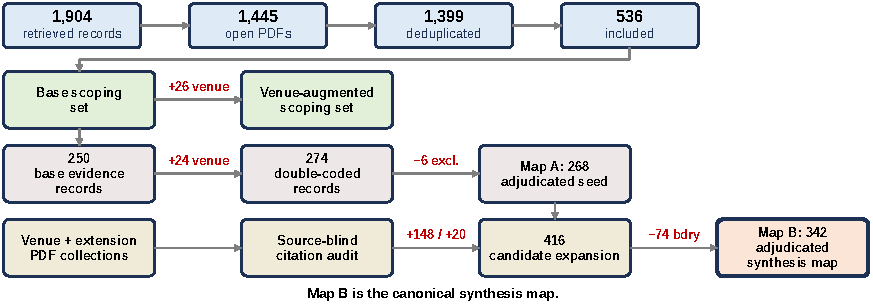
\includegraphics[width=\textwidth]{figures/generated/fig_corpus_lineage.pdf}%
\caption{Corpus lineage. Red deltas on the connectors are, in order, $+26$ and
$+24$ venue-linked additions, $-6$ exclusions, $+148$ new and $+20$ enriched
rows from the citation audit, and $-74$ boundary rows removed at adjudication.
The 416-row venue-expanded candidate map is second-coded and adjudicated into
Map~B (342 rows), the canonical synthesis evidence map. Map~A (268 rows) is the
double-coded adjudicated seed used for IAA and adjudication audit; the base and
venue-augmented scoping sets are used only for boundary checks, while a separate
300-paper source-blind citation audit over the venue and extension PDF
collections decides which papers enter the main text, case studies, or
appendix.}
\label{fig:corpus-flow}
\end{figure*}

\begin{table*}[t]
\centering
\small
\begin{tabularx}{\linewidth}{p{0.18\linewidth}p{0.16\linewidth}X}
\toprule
\textbf{Stage} & \textbf{Count} & \textbf{Rule} \\
\midrule
Initial retrieval & 1,904 records & Keyword search over arXiv, ACL Anthology, OpenReview, USENIX, AAAI/ACM landing pages where open versions were available, plus curated robust/trustworthy RAG paper lists; search cutoff 2026-06-03. \\
Open full-text corpus & 1,445 PDFs & Downloaded only open PDFs; removed failed downloads, inaccessible files, and non-PDF artifacts. \\
Deduplicated candidates & 1,399 papers & Deduplicated by normalised title and arXiv/proceedings identifiers; retained the most complete metadata record when preprint and proceedings versions overlapped. \\
Relevance screening & 536 included papers & Included papers that study RAG robustness, reliability, uncertainty, calibration, faithfulness, attack/defense, or evaluation under unreliable evidence; excluded application-only RAG papers. \\
Core pool & 112 papers & Papers directly shaping the taxonomy, threat/failure model, intervention mechanisms, or evaluation framework. \\
Core reading set & 100 papers & Core papers used as main narrative anchors; the remaining 12 core-pool papers stay in the broader scoping set. \\
Base scoping set & 300 papers & Core papers plus representative supporting work across all taxonomy branches before venue follow-up triage. \\
Venue-augmented scoping set & 326 papers & Base scoping set plus 26 venue-linked additions after follow-up triage. \\
Candidate evidence records & 274 papers & Base evidence map of 250 papers plus 24 venue-linked additions, double-coded and adjudicated. \\
Map A adjudicated seed & 268 papers & Candidate evidence records retained after final adjudication; used for IAA/adjudication provenance. \\
Map-B candidate expansion & 416 papers & Map A plus 148 source-blind human-citation-audit additions and 20 enriched original rows; used for second-coding review. \\
Map B adjudicated synthesis map & 342 papers & Map A plus 74 retained additions after second coding and final adjudication; frozen for current descriptive statistics. Post-freeze discoveries enter a recall log until a new version is coded. \\
\bottomrule
\end{tabularx}
\caption{Screening-flow summary. Search ends on 2026-06-03; coding and adjudication artifacts freeze on 2026-06-15. The supplement provides query strings, source counts, rules, exclusions, hashes, and a post-freeze recall log.}
\label{tab:review-protocol}
\end{table*}

\begin{table*}[t]
\centering
\scriptsize
\renewcommand{\arraystretch}{0.9}
\begin{tabularx}{\linewidth}{>{\raggedright\arraybackslash}p{0.22\linewidth}>{\raggedright\arraybackslash}p{0.16\linewidth}>{\raggedright\arraybackslash}p{0.25\linewidth}X}
\toprule
\textbf{Map-B field group} & \textbf{Coverage} & \textbf{Coding / audit source} & \textbf{Use and caveat} \\
\midrule
Canonical identifiers and source flags & 342/342 title, year, URL, source stratum, Map-A membership, Map-B version, core-reading flag & Deterministic merge from Map A, the venue/extension pools manifests, source-blind citation-audit decisions, and second-coding adjudication. & Defines the canonical adjudicated row set and source strata. \\
Core taxonomy fields & 342/342 failure type, taxonomy categories, method family, intervention point, contribution note, limitation note & Map-A adjudicated labels for original rows; second coding adjudicated labels for retained additions. & Used for Map-B synthesis and sensitivity counts. \\
Task / metric metadata & High coverage after adjudication & Map-A labels plus human-audit rationales and manifest metadata for retained additions. & Missing rows are not imputed for metric-level claims. \\
Author / venue metadata & Source/venue strata complete; author metadata incomplete for some additions & Proceedings metadata and paper manifests. & Venue/source strata are complete; author normalization remains an artifact-release cleanup item. \\
Human-audited rows retained in Map B & 94 retained rows with human citation-audit metadata & 74 retained additions plus 20 enriched Map-A rows. & Citation-audit metadata supports source-stratified synthesis; 74 excluded candidate additions remain in the release as boundary rows. \\
Second-coding/adjudication boundary & Map A: 274 candidates $\rightarrow$ 268 adjudicated rows; Map-B additions: 148 candidates $\rightarrow$ 74 retained additions & Map A has two-source independent coding and final adjudication; Map-B additions have independent second coding and final adjudication. & Second-coding agreement is strong, and adjudication is now applied to the canonical 342-row Map B. \\
\bottomrule
\end{tabularx}
\caption{Coding protocol and field coverage for the 342-row adjudicated Map B. The table separates Map-A adjudicated IAA, source-blind citation-audit metadata, and the second-coding/adjudication pass over the 148 candidate additions.}
\label{tab:map-b-coding-coverage}
\end{table*}

\begin{table*}[t]
\centering
\scriptsize
\renewcommand{\arraystretch}{0.92}
\begin{tabularx}{\linewidth}{>{\raggedright\arraybackslash}p{0.20\linewidth}>{\raggedright\arraybackslash}p{0.15\linewidth}>{\raggedright\arraybackslash}p{0.30\linewidth}X}
\toprule
\textbf{Artifact / set} & \textbf{Count} & \textbf{Count definition} & \textbf{Use in this paper} \\
\midrule
Map-A double-coded candidates & 274 & Candidate records coded by two human sources before final inclusion adjudication. & Used for human-human agreement and adjudication; six records were excluded from Map A. \\
Map A adjudicated seed & 268 & Included records after adjudication: 42 venue/proceedings-linked, 222 arXiv-only or emerging preprints, 2 preprints with year tags, 1 review-platform record, and 1 other/uncategorized record. & Used as the IAA/adjudication provenance snapshot, not the current synthesis denominator. \\
Venue-augmented scoping set & 326 & Original base scoping set plus 26 triaged venue-linked additions. & Used for broader scoping and boundary checks; not all rows are evidence-map records. \\
Source-blind citation audit & 300 & Human citation decisions over venue PDFs and extension PDFs. & Determines which audited papers enter the main text, case studies, appendix, background, or exclusion set; distinct from the base scoping set. \\
Map-B candidate expansion & 416 & Map A plus 148 candidate additions supported by the source-blind citation audit; 20 original rows enriched with citation-audit metadata. & Pre-adjudication expansion candidate map used for second-coding review. \\
Map B adjudicated synthesis map & 342 & Map A plus 74 retained additions after second coding and final adjudication. & Current evidence map for source-stratified synthesis and Map-B cross-tabs. \\
\bottomrule
\end{tabularx}
\caption{Reconciliation of reported corpus counts. The 342-row adjudicated Map B is the canonical synthesis map; Map A and the 274-candidate set are retained to report double-coding and adjudication provenance.}
\label{tab:source-strata-reconciliation}
\end{table*}


\FloatBarrier
\end{document}
